\documentclass[../include.tex]{subfiles}
\begin{document}
\section{Introduction}
\par There is only a relatively small number of cases, when we can find an analytical solution for a differential equation. Therefore the development of numerical methods for finding approximate solutions with the desired accuracy is very important. For solving partial differential equations, several numerical methods have been developed. Among the most popular numerical techniques are the finite difference method, the finite volume method and the finite element method. These methods reduce the problem of solving a differential equation to solving a system of equations. Below we give a brief description of these methods for the 1D case, which is relevant to this work.

The finite difference method \cite{lev_fdm} is the oldest and in some ways the simplest approach. The idea is to replace derivatives with differences. The domain of interest is divided into a given number of elements connected by nodes. The differences are calculated from the approximations at the nodes. The way, in which we calculate the differences come from accuracy and stability considerations. The method is well suited for regular rectangular meshes, but becomes impractical for complicated domains, which are often the subject of interest in applications.

The finite volume method uses a different approach \cite{lev, patankar}. First we subdivide our spatial domain of interest into "finite volumes" or grid cells. In 1D these are intervals on the real line. We denote the $ i $-th grid cell by
\[
p_i = (x_{i-1/2}, x_{i+1/2}).
\]
The method is based on the conservation of a quantity $ u(t, x) $. Instead of looking for approximations of the values of $ u $ at the nodes, as we do in the finite difference method, we are interested in the approximations of the integral of $ u $ over each interval. We assume that the change of the integral over a time interval $ [t^{n-1}, t^{n}] $ for $ n=1,2,... $ is due to the fluxes $ f(t, x) $ at the endpoints of the cells:
\begin{equation}
	\label{conservation_integral}
	\int_{p_i} u(t^{n}, x) \,\mathrm{d}x - \int_{p_i} u(t^{n-1}, x) \,\mathrm{d}x = 
\int_{t^{n-1}}^{t^{n}} f(t, x_{i-1/2}) \,\mathrm{d}t - \int_{t^{n-1}}^{t^{n}} f(t, x_{i+1/2}) \,\mathrm{d}t.
\end{equation}
Our goal is to calculate how the average of $ u $ changes over time, i.e. if we know the integral at time $ t^{n-1} $, what is its value at a later time $ t^{n} $.
For this purpose we approximate the average value of $ u $ by a constant representative value denoted as $ \bar{u}_i^{n-1} $ inside the $ i $-th cell at time $ t^{n-1} $. The approximation of the integral becomes
\[
\int_{p_i} u(t^{n-1}, x) \,\mathrm{d}x \approx \bar{u}_i^{n-1}\, h,
\]
where  $ h = x_{i+1/2} - x_{i-1/2} $ is the length of a cell.
We can also express
\[
\int_{t^{n-1}}^{t^{n}} f(t, x_{i-1/2}) \,\mathrm{d}t \approx F_{i-1/2}\, \tau,
\]
where $ F_{i-1/2} $ is an approximation of the average flux at $ x_{i-1/2} $ and over time interval $ [t^{n-1}, t^{n}] $ with $ \tau = t^{n} - t^{n-1} $.
After substitution the conservation law takes the form
\[
(\bar{u}_i^{n} - \bar{u}_i^{n-1}) h = (F_{i-1/2} -  F_{i+1/2}) \tau
\]
Dividing by the length of the cell $ h $, rearranging terms we get an expression for the approximate average value at time $ t^{n} $ as
\begin{equation}
	\label{finite_volume}
	\bar{u}_i^{n} = \bar{u}_i^{n-1} - \frac{\tau}{h}(F_{i+1/2} - F_{i-1/2}).
\end{equation}
If we assume dependence of the flux at a given interface on the representative values in the neighboring cells in space and time we get a fully discrete method. The scheme \eqref{finite_volume} has a discrete conservation property, which we can see by summing $ \bar{u}_i^{n}\, h $, the approximation of the integral of a quantity $ u $, over any set of cells
\[
h \sum_{i=I}^{J} \bar{u}_i^{n} = h \sum_{i=I}^{J} \bar{u}_i^{n-1} - \tau\sum_{i=I}^{J}\left(F_{i+1/2} - F_{i-1/2}\right).
\]
It can be seen, that the terms in the sum of fluxes on the right-hand side cancel out, except the fluxes at the boundaries $ I $ and $ J $, i.e.\
\[
h \sum_{i=I}^{J} \bar{u}_i^{n} = h \sum_{i=I}^{J} \bar{u}_i^{n-1} - \tau\left(F_{J+1/2} - F_{I-1/2}\right).
\]
The scheme is said to be in conservation form, because it mimics the property of the conservation law \eqref{conservation_integral}, i.e.\ the change of a quantity inside an interval is due to fluxes at the endpoints. This property makes the method well suited for solving conservation laws. Unlike the finite difference method, it can be used even for complicated domains.

A very successful method for solving differential equations is the finite element method \cite{reddy, olv}. Similarly as in the case of the previous methods, we subdivide the domain of interest into smaller pieces, finite elements. It is based either on a minimization principle, if possible, or on the concept of a weak solution to a differential equation. It is well suited for complicated geometries similarly to the finite volume method.

In this work we apply the inflow-implicit\slash outflow-explicit (IIOE) scheme to advection terms of the nonlinear equations discussed in the previous chapter. The method is based on finite volume space discretization and a semi-implicit discretization in time. Inflows to the cells are treated implicitly and outflows are treated explicitly. We could explain this idea intuitively that we know what is flowing out from a cell at a given time but leave the method to solve a system of equations determined by the inflows to obtain the solution values at the new time step. In earlier works, \cite{iioe2012, iioe2} it was shown that the IIOE scheme is formally second order accurate in space and time for 1D linear advection problems with variable velocity. In this work, we show that the IIOE method is formally second order consistent also in case of nonlinear scalar conservation laws for smooth solutions. Combining with the Crank-Nicolson scheme for the diffusion term, we get a new numerical scheme for the nonlinear advection-diffusion problem (\ref{burg}). We also present a limited IIOE scheme for inviscid conservation laws, which is important for problems, where solutions tend to develop shocks.
%====================================================================================================================================================
\section{Advection with variable velocity}

For reader convenience we present here the derivation of the IIOE scheme as in \cite{iioe0,iioe1,iioe2012,iioe2} for the equation
\begin{equation}
	u_t + vu_x = 0, 
	\label{adv}
\end{equation}
where $ v = v(x) $. We rewrite (\ref{adv}) in the equivalent form
\begin{equation}
	u_t + (vu)_x - uv_x = 0,
	\label{adv1}
\end{equation}
and integrating over a grid cell $ p_i $ with cell center $ x_i $, length $ h $, left border $ x_{i-\frac{1}{2}} $, right border $ x_{i+\frac{1}{2}} $ yields
\[ \int_{p_i} u_t\, dx + 
\int_{p_i}(vu)_x\, dx - 
\int_{p_i} uv_x\, dx = 0\]
Let us denote $ v_i = v(x_i) $, $ v_{i - \frac{1}{2}} = v(x_{i-\frac{1}{2}}) $, $ v_{i + \frac{1}{2}} = v(x_{i+\frac{1}{2}}) $. Let us denote by $ u_i^n $ a value of the solution inside the $ i $-th finite volume cell at time step $ n $ computed by the numerical scheme. We use a constant representation of the solution inside a cell $ p_i $ denoted by $ \bar u_i $ and constant representative values at the cell interfaces denoted by $ \bar u_{i - \frac{1}{2}} $, $ \bar u_{i + \frac{1}{2}} $ respectively. Using the Newton-Leibniz formula we obtain
\[ \int_{p_i} u_t\, dx +
v_{i + \frac{1}{2}} \bar u_{i + \frac{1}{2}} - v_{i - \frac{1}{2}} \bar u_{i - \frac{1}{2}} - 
\bar u_i (v_{i + \frac{1}{2}} - v_{i - \frac{1}{2}}) = 0. \]
By rearranging terms we get
\[\int_{p_i} u_t\, dx + 
v_{i - \frac{1}{2}}(\bar u_i - \bar u_{i - \frac{1}{2}}) + (-v_{i + \frac{1}{2}})(\bar u_i - \bar u_{i + \frac{1}{2}}) = 0.\]
$ v_{i - \frac{1}{2}} > 0 $ represents inflow from the left cell interface, while $ (-v_{i + \frac{1}{2}}) > 0 $ represents inflow from the right cell interface. Otherwise they represent outflows. Thus we define
\begin{align}
	a^{in}_{i-\frac{1}{2}} &= \textrm{max}(v_{i-\frac{1}{2}},0),\quad 
	a^{out}_{i-\frac{1}{2}} = \textrm{min}(v_{i-\frac{1}{2}},0), 
	\\
	a^{in}_{i+\frac{1}{2}} &= \textrm{max}(-v_{i+\frac{1}{2}},0),\, 
	a^{out}_{i+\frac{1}{2}} = \textrm{min}(-v_{i+\frac{1}{2}},0). 
\end{align}
We use a simple finite difference approximation for the time derivative $ \frac{u^n_i - u^{n-1}_i}{\tau} $,
where $ \tau $ is a uniform time step, take inflow implicitly, outflow explicitly and use the straightforward reconstructions $ \bar u_i^n = u^n_i $, $ \bar u_{i - \frac{1}{2}}^n = \frac{1}{2} (u_i^n + u_{i-1}^n) $, $ \bar u_{i + \frac{1}{2}}^n = \frac{1}{2} (u_i^n + u_{i+1}^n) $, we obtain the basic one-dimensional IIOE scheme for variable velocity:
\begin{eqnarray}
	\label{iioe0}
	u^n_i + \frac{\tau}{2h} a^{in}_{i-\frac{1}{2}}  \left(u^n_i - u^n_{i-1}\right) + 
	\frac{\tau}{2h} a^{in}_{i+\frac{1}{2}} \left(u^n_i - u^n_{i+1}\right) = \\
	u^{n-1}_i - \frac{\tau}{2h} \left(a^{out}_{i-\frac{1}{2}} \left(u^{n-1}_i - u^{n-1}_{i-1}\right) + 
	a^{out}_{i+\frac{1}{2}} \left(u^{n-1}_i - u^{n-1}_{i+1}\right)\right).\nonumber
\end{eqnarray}
%====================================================================================================================================================
\section{Nonlinear advection with diffusion}

We can extend these ideas for velocities depending on the solution. For the advective part of the viscous Burgers' equation (\ref{burg}) we calculate the velocities from the solution at the cell interfaces. This leads us to a nonlinear system of equations, which we solve iteratively. The time dependent velocities in the $ k $-th iteration become
\[ v^{n,k}_{i-\frac{1}{2}} = (u^{n,k-1}_i + u^{n,k-1}_{i-1})\slash 2,\quad
v^{n,k}_{i+\frac{1}{2}} = (u^{n,k-1}_i + u^{n,k-1}_{i+1})\slash 2,\quad k=1,2,3,.... \]
and $ u^{n,0}_i = u^{n-1}_i $.

When solving the traffic flow problem (\ref{traffic}), we replace $ u^n_i $ by $ \rho^n_i $. Considering that characteristic speed in the equations of traffic flow \eqref{traffic} equals $ 1-2\rho $, using the same reconstructions as for $ u^n_i $ and cancelling common factors, for $ v_{max} = 1 $ the time dependent velocities according to (\ref{u-ro}) in the $ k $-th iteration become
\[ v^{n,k}_{i-\frac{1}{2}} = 1 - (\rho^{n,k-1}_i + \rho^{n,k-1}_{i-1}),\quad
v^{n,k}_{i+\frac{1}{2}} = 1 - (\rho^{n,k-1}_i + \rho^{n,k-1}_{i+1}). \]
In both cases we consider the time dependent splitting to inflows and outflows
\begin{align}
	a^{in,n-1}_{i-\frac{1}{2}} &= \textrm{max}(\mathrm{sgn}(v^{n-1}_{i-\frac{1}{2}}),0),\quad 
	a^{out,n-1}_{i-\frac{1}{2}} = \textrm{max}(\mathrm{sgn}(-v^{n-1}_{i-\frac{1}{2}}),0), 
	\\
	a^{in,n-1}_{i+\frac{1}{2}} &= \textrm{min}(\mathrm{sgn}(v^{n-1}_{i+\frac{1}{2}}),0),\quad
	a^{out,n-1}_{i+\frac{1}{2}} = \textrm{min}(\mathrm{sgn}(-v^{n-1}_{i+\frac{1}{2}}),0). 
\end{align}
In order to keep second order accuracy of the IIOE scheme, the diffusion part is treated
by the Crank-Nicolson approach. Finally we end up with the following system
\begin{eqnarray}
	\label{iioe}
	u^{n,k}_i + \frac{\tau}{2h} \left(a^{in,n-1}_{i-\frac{1}{2}} v^{n,k}_{i-\frac{1}{2}} + \frac{\sigma}{h} \right) \left(u^{n,k}_i - u^{n,k}_{i-1}\right) + 
	\frac{\tau}{2h} \left(a^{in,n-1}_{i+\frac{1}{2}} v^{n,k}_{i+\frac{1}{2}} + \frac{\sigma}{h} \right) \left(u^{n,k}_i - u^{n,k}_{i+1}\right) = \\
	u^{n-1}_i - \frac{\tau}{2h} \left(\left(a^{out,n-1}_{i-\frac{1}{2}} v^{n-1}_{i-\frac{1}{2}}  + \frac{\sigma}{h} \right) \left(u^{n-1}_i - u^{n-1}_{i-1}\right) + 
	\left(a^{out,n-1}_{i+\frac{1}{2}} v^{n-1}_{i+\frac{1}{2}} + \frac{\sigma}{h} \right) \left(u^{n-1}_i - u^{n-1}_{i+1}\right)\right),\nonumber
\end{eqnarray}
which we solve iteratively. In every iteration, we calculate the residuum defined as
\[ \frac{1}{N}||A(u^{n,k})u^{n,k} - Bu^{n-1}||, \]
where $ A(u^{n,k}) $ and $ B $ are coefficient matrices obtained by writing the system (\ref{iioe}) using matrix notation and $ N $ is the number of unknowns. Our goal was to reach second order accuracy. For this purpose, while solving the Burgers' equation (\ref{burg}), it is sufficient to stop doing iterations when the residuum drops below $ 10^{-6} $. To achieve the desired accuracy for the traffic flow problem (\ref{traffic}), we stopped the calculation when the residuum drops below $ 10^{-7} $. It  means that we have to solve few times (usually from 3 to 6) a tridiagonal system in every time step of the IIOE scheme in case of nonlinear advection-diffusion problems. The tridiagonal system is solved using the Thomas' algorithm. All the numerical experiments are performed on a bounded interval, at the endpoints we have Dirichlet boundary conditions, calculated from the exact solutions at every time step.
%====================================================================================================================================================
\subsection{Numerical experiments - viscous Burgers' equation}
In order to test the numerical scheme \eqref{iioe}, we chose 4 representative solutions of the viscous Burgers' equation:
the traveling-wave solution, the rarefaction-wave solution, the triangular-wave solution and a trigonometric solution. In an earlier work \cite{iioe0} the authors have used the traveling-wave solution to test the numerical scheme similar to (\ref{iioe}). These experiments were already presented in \cite{algoritmy}.

\textbf{Traveling wave.} The traveling-wave solution can be obtained by looking for special solutions of the Burgers' equation (\ref{burg}) that are only shifted in time. This way we can obtain, see, e.g.\ \cite{olv}
\begin{equation}
	u(t,x) = u_r + \frac{1}{2}(u_l-u_r)\left(1-\tanh \left(\frac{(u_l-u_r)(x-st)}{4 \sigma}\right) \right),
	\label{travel}
\end{equation}
where $ s = (u_l + u_r)/2 $ is the propagation speed. Here we chose $ u_l = 1,\,u_r = 0 $. We will use it as our first example to test the numerical scheme (\ref{iioe}) on space interval $ (-0.5, 0.5) $ and time interval $ (0, 0.48) $.
First we solve the problem with $ \sigma = 0.01 $.
In this test example we chose a time step $ \tau = 4h $. It means that for $ h = 0.01 (n = 100) $ we use a time step $ \tau = 0.04 $. Then one can refine the time step and grid size in order to check that the scheme is second order accurate, cf. Table \ref{tab:travel}. The visual comparisons of the numerical and exact solutions for $ n = 100 $ are presented in Figure \ref{fig:travel}.

It is interesting to consider what happens if we do not perform any nonlinear iteration. Which means that we calculate the inflow coefficients using the values of the solution from the previous time step. This way we get EOC = 1, as it is documented in Table \ref{tab:travel_1iter}. In Figure \ref{fig:travel_iter} we can observe that the propagation speed of the numerical solution differs from the exact one. By refining the grid, the speed gets closer to the exact one.

In the second case we decreased the viscosity to $ \sigma = 0.001 $. In Table \ref{tab:travelsig1/1000} we show errors and EOC for refined and coarsened grids and time step. One can again see that EOC = 2 also in this example when refining the grid. The lower convergence rate in the beginning is caused by oscillations when the grid size is not sufficiently fine, but as we can see from Figure \ref{fig:travel_sig1/1000_n500} these oscillations are ”stable”, they do not increase in time and
by refining the spatial resolution they are removed completely as documented in Figure \ref{fig:travel_sig1/1000_n1000}.

\begin{table}[ht]
	\caption{Report on the $L_2$ errors of $\mathrm{IIOE}$ method for the traveling-wave solution {\rm (\ref{travel})} of the viscous Burgers' equation {\rm (\ref{burg})} with $\sigma = 0.01$. }
	\begin{center} \footnotesize
		\begin{tabular}{|c|c|c|c|c|c|}
			\hline  
			$ n $ & $ h $ & $\tau$ & NTS & $L_2(I,L_2)$ & EOC\\
			\hline
			\lower.3ex\hbox{100} & \lower.3ex\hbox{0.01} & \lower.3ex\hbox{0.04} & \lower.3ex\hbox{12} & \lower.3ex\hbox{5.0 $10^{-3}$} &\\
			\hline
			\lower.3ex\hbox{200} & \lower.3ex\hbox{0.005} & \lower.3ex\hbox{0.02} & \lower.3ex\hbox{24} & \lower.3ex\hbox{1.22 $10^{-3}$} & \lower.3ex\hbox{2.03}\\
			\hline
			\lower.3ex\hbox{400} & \lower.3ex\hbox{0.0025} & \lower.3ex\hbox{0.01} & \lower.3ex\hbox{48} & \lower.3ex\hbox{3.03 $10^{-4}$} & \lower.3ex\hbox{2.01}\\
			\hline
			\lower.3ex\hbox{800} & \lower.3ex\hbox{0.00125} & \lower.3ex\hbox{0.005} & \lower.3ex\hbox{96} & \lower.3ex\hbox{7.74 $10^{-5}$} & \lower.3ex\hbox{1.97}\\
			\hline
			\lower.3ex\hbox{1600} & \lower.3ex\hbox{0.000625} & \lower.3ex\hbox{0.025} & \lower.3ex\hbox{192} & \lower.3ex\hbox{1.90 $10^{-5}$} & \lower.3ex\hbox{2.02}\\
			\hline
		\end{tabular}
	\end{center}
	\label{tab:travel}
\end{table}

\begin{figure}[h!]
	\centering
	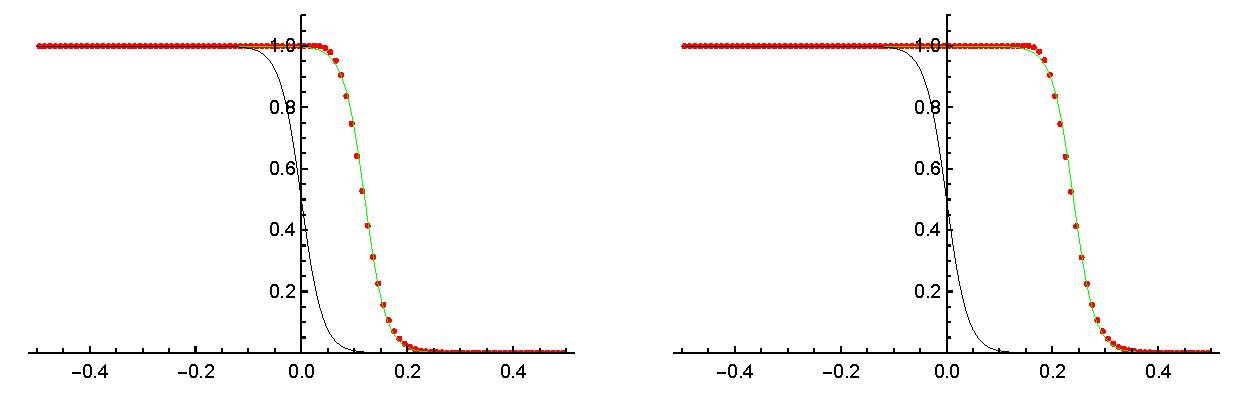
\includegraphics[width=\textwidth]{figures/travel100.pdf}
	\caption{Comparing the $ \mathrm{IIOE} $ scheme with the exact traveling-wave solution {\rm (\ref{travel})} in time $ t=0.24 $ (left) and $ t = 0.48 $ (right), with $ \sigma=0.01 $, $ n=100 $, $ \tau=4h $}
	\label{fig:travel}
\end{figure}

\begin{table}[h!]
	\caption{Report on the $L_2$ errors of $\mathrm{IIOE}$ method for the traveling-wave solution {\rm (\ref{travel})} of the viscous Burgers' equation {\rm (\ref{burg})} with $\sigma = 0.01$, number of nonlinear iterations = 1. }
	\begin{center} \footnotesize
		\begin{tabular}{|c|c|c|c|c|c|}
			\hline  
			$ n $ & $ h $ & $\tau$ & NTS & $L_2(I,L_2)$ & EOC\\
			\hline
			\lower.3ex\hbox{100} & \lower.3ex\hbox{0.01} & \lower.3ex\hbox{0.04} & \lower.3ex\hbox{12} & \lower.3ex\hbox{4.41 $10^{-2}$} &\\
			\hline
			\lower.3ex\hbox{200} & \lower.3ex\hbox{0.005} & \lower.3ex\hbox{0.02} & \lower.3ex\hbox{24} & \lower.3ex\hbox{2.32 $10^{-2}$} & \lower.3ex\hbox{0.93}\\
			\hline
			\lower.3ex\hbox{400} & \lower.3ex\hbox{0.0025} & \lower.3ex\hbox{0.01} & \lower.3ex\hbox{48} & \lower.3ex\hbox{1.18 $10^{-2}$} & \lower.3ex\hbox{0.97}\\
			\hline
			\lower.3ex\hbox{800} & \lower.3ex\hbox{0.00125} & \lower.3ex\hbox{0.005} & \lower.3ex\hbox{96} & \lower.3ex\hbox{5.96 $10^{-3}$} & \lower.3ex\hbox{0.99}\\
			\hline
		\end{tabular}
	\end{center}
	\label{tab:travel_1iter}
\end{table}

\begin{figure}[h!]
	\centering
	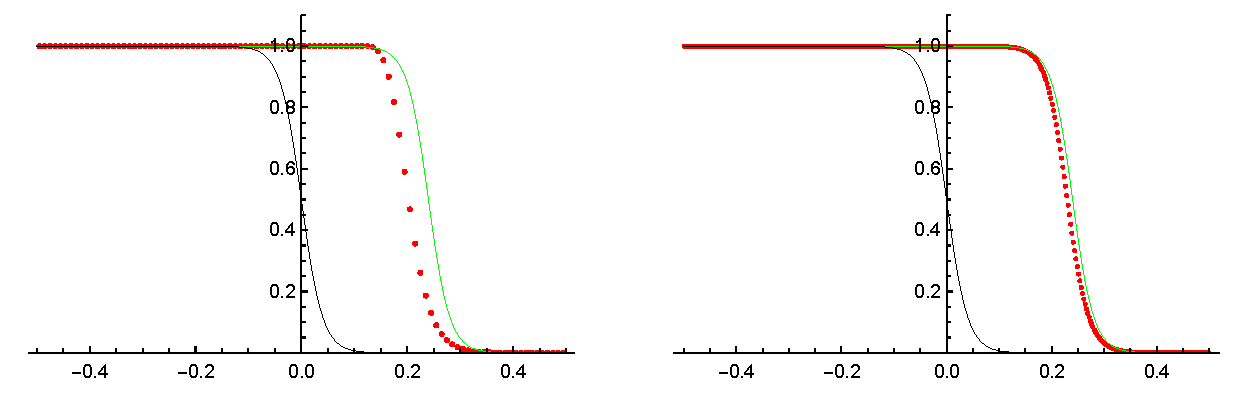
\includegraphics[width=\textwidth]{figures/traveliter}
	\caption{Comparing the $ \mathrm{IIOE} $ scheme with the exact traveling-wave solution {\rm (\ref{travel})} in time $ t=0.48 $, with $ \sigma=0.01 $, $ n=100 $(left), $ n=400 $(right), $ \tau=4h $, $ \textrm{number of nonlinear iterations} = 1 $. We can see that after refining the grid, the propagation speed of the numerical solution is getting closer to the exact speed.}
	\label{fig:travel_iter}
\end{figure}

\begin{table}[h!]
	\caption{Report on the $L_2$ errors of $\mathrm{IIOE}$ method for the traveling-wave solution {\rm (\ref{travel})}  of the viscous Burgers' equation {\rm (\ref{burg})}  with $\sigma = 0.001$. }
	\begin{center} \footnotesize
		\begin{tabular}{|c|c|c|c|c|c|}
			\hline  
			$ n $ & $ h $ & $\tau$ & NTS & $L_2(I,L_2)$ & EOC\\
			\hline
			\lower.3ex\hbox{250} & \lower.3ex\hbox{0.004} & \lower.3ex\hbox{0.016} & \lower.3ex\hbox{30} & \lower.3ex\hbox{2.01 $10^{-2}$} &\\
			\hline
			\lower.3ex\hbox{500} & \lower.3ex\hbox{0.002} & \lower.3ex\hbox{0.08} & \lower.3ex\hbox{60} & \lower.3ex\hbox{6.84 $10^{-3}$} & \lower.3ex\hbox{1.55}\\
			\hline
			\lower.3ex\hbox{1000} & \lower.3ex\hbox{0.001} & \lower.3ex\hbox{0.04} & \lower.3ex\hbox{120} & \lower.3ex\hbox{1.79 $10^{-3}$} & \lower.3ex\hbox{1.94}\\
			\hline
			\lower.3ex\hbox{2000} & \lower.3ex\hbox{0.0005} & \lower.3ex\hbox{0.02} & \lower.3ex\hbox{240} & \lower.3ex\hbox{4.55 $10^{-4}$} & \lower.3ex\hbox{1.97}\\
			\hline
		\end{tabular}
	\end{center}
	\label{tab:travelsig1/1000}
\end{table}

\begin{figure}[h!]
	\centering
	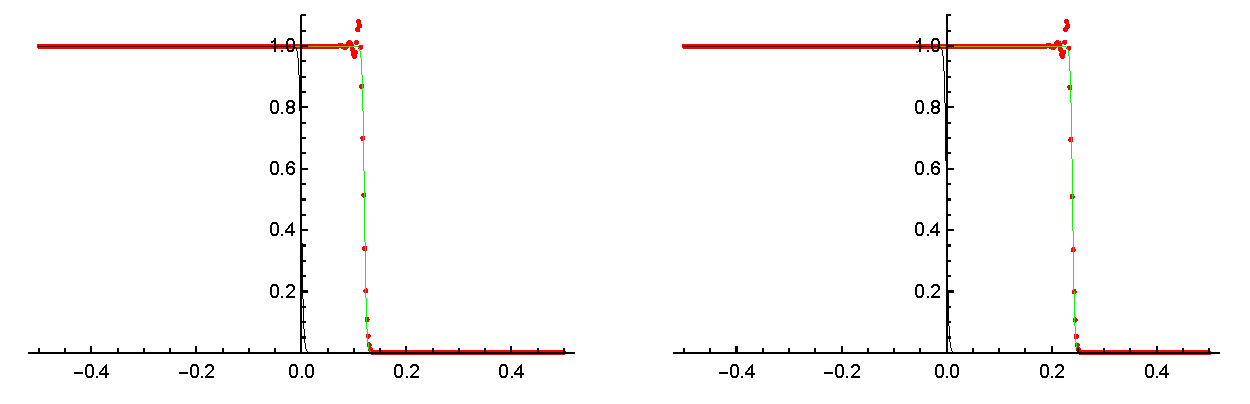
\includegraphics[width=\textwidth]{figures/travelsig0015002448}
	\caption{Comparing the $ \mathrm{IIOE} $ scheme with the exact traveling-wave solution {\rm (\ref{travel})} in time $ t=0.24 $ (left) and $ t = 0.48 $ (right), with $ \sigma=0.001 $, $ n=500 $, $ \tau=4h $. We can observe small nonincreasingly propagating oscillations.}
	\label{fig:travel_sig1/1000_n500}
\end{figure}

\begin{figure}[h!]
	\centering
	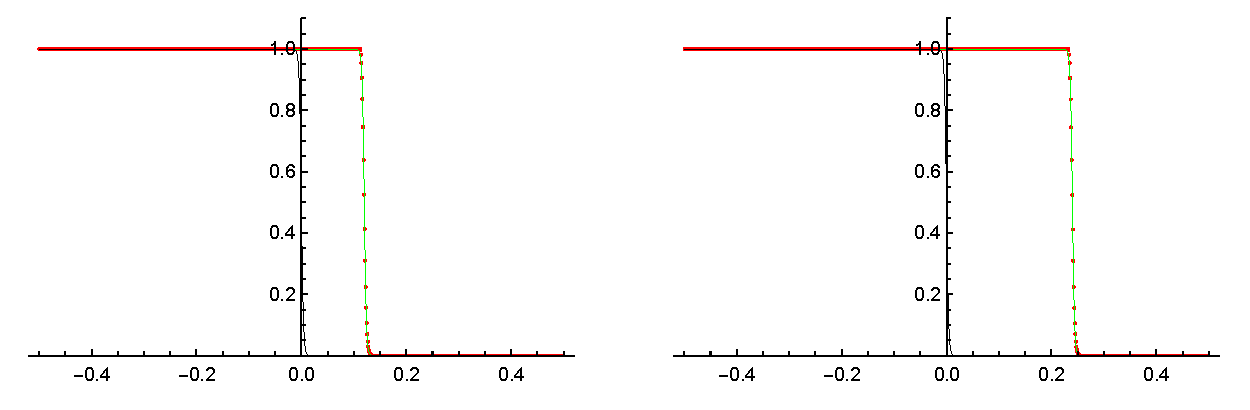
\includegraphics[width=\textwidth]{figures/travelsig0011000024048}
	\caption{Comparing the $ \mathrm{IIOE} $ scheme with the exact traveling-wave solution {\rm (\ref{travel})} in time $ t=0.24 $ (left) and $ t = 0.48 $ (right), with $ \sigma=0.001 $, $ n=1000 $, $ \tau=4h $. On the refined grid the oscillations are gone.}
	\label{fig:travel_sig1/1000_n1000}
\end{figure}
%====================================================================================================================================================
\newpage
\textbf{Rarefaction wave.} The next example is the rarefaction-wave solution \eqref{rare}. We chose $ u_l = 0,\,u_r = 1 $ and $ \sigma = 0.01 $. First, equation (\ref{burg}) is solved by the scheme (\ref{iioe}) on space interval $ (-0.5, 0.5) $ and time interval $ [0.01, 0.41) $. Since the exact solution (\ref{rare}) is defined for $ t>0 $, we decided to initialize the calculation at time 0.01. The time step $ \tau $ was chosen to be equal to $ 4h $ again. The numerical solution is visually compared to the exact solution in Figure \ref{fig:rare}. The errors are presented in Table \ref{tab:rare}.

\begin{table}[h!]
	\caption{Report on the $L_2$ errors of $\mathrm{IIOE}$ method for the rarefaction-wave solution {\rm (\ref{rare})} of the viscous Burgers' equation {\rm (\ref{burg})} with $\sigma = 0.01$. }
	\begin{center} \footnotesize
		\begin{tabular}{|c|c|c|c|c|c|}
			\hline  
			$ n $ & $ h $ & $\tau$ & NTS & $L_2(I,L_2)$ & EOC\\
			\hline
			\lower.3ex\hbox{100} & \lower.3ex\hbox{0.01} & \lower.3ex\hbox{0.04} & \lower.3ex\hbox{10} & \lower.3ex\hbox{5.48 $10^{-3}$} &\\
			\hline
			\lower.3ex\hbox{200} & \lower.3ex\hbox{0.005} & \lower.3ex\hbox{0.02} & \lower.3ex\hbox{20} & \lower.3ex\hbox{1.56 $10^{-3}$} & \lower.3ex\hbox{1.82}\\
			\hline
			\lower.3ex\hbox{400} & \lower.3ex\hbox{0.0025} & \lower.3ex\hbox{0.01} & \lower.3ex\hbox{40} & \lower.3ex\hbox{4.01 $10^{-4}$} & \lower.3ex\hbox{1.96}\\
			\hline
			\lower.3ex\hbox{800} & \lower.3ex\hbox{0.00125} & \lower.3ex\hbox{0.005} & \lower.3ex\hbox{80} & \lower.3ex\hbox{1.00 $10^{-4}$} & \lower.3ex\hbox{2.00}\\
			\hline
		\end{tabular}
	\end{center}
	\label{tab:rare}
\end{table}

\begin{figure}[h!]
	\centering
	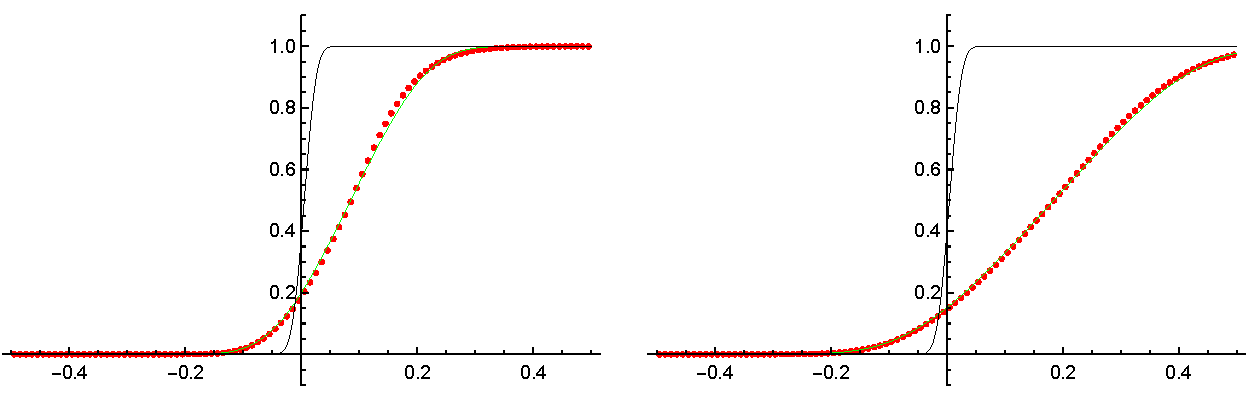
\includegraphics[width=\textwidth]{figures/rare100}
	\caption{Comparing the $\mathrm{IIOE}$ scheme with the exact rarefaction-wave solution {\rm (\ref{rare})} in time $ t=0.17 $ (left) and $ t = 0.41 $ (right), with $ \sigma=0.01 $, $ n=100 $, $ \tau=4h $}
	\label{fig:rare}
\end{figure}
%====================================================================================================================================================
\newpage
\textbf{Triangular wave.} Our third example is the triangular-wave solution \eqref{triang}. In this case the problem (\ref{burg}) is solved by the scheme (\ref{iioe}) on space interval $ (-0.5, 1.5) $ and time interval $ (0.01, 0.51) $ with $ \sigma = 0.02 $. Again, the exact solution (\ref{triang}) is defined for $ t > 0 $ so the numerical calculation was initialized at time 0.01. In Table \ref{ttri} we show the errors for refined grids and time step. When the grid size is not sufficiently fine, we can observe oscillations at the peak of the wave in Figure ~\ref{fig:triang-osc}. These oscillations do not grow unbounded and can be removed by refining the grid as it is shown in Figure ~\ref{fig:triang}.

\begin{table}[ht]
	\caption{Report on the $L_2$ errors of $\mathrm{IIOE}$ method for the triangular-wave solution {\rm (\ref{triang})} of the viscous Burgers' equation {\rm (\ref{burg})} with $\sigma = 0.02$. }
	\begin{center} \footnotesize
		\begin{tabular}{|c|c|c|c|c|c|}
			\hline  
			$n$ & $h$ & $\tau$ & \lower.3ex\hbox{NTS} & \lower.3ex\hbox{$L_2(I,L_2)$} & \lower.3ex\hbox{EOC}\\
			\hline
			\lower.3ex\hbox{100} & \lower.3ex\hbox{0.02} & \lower.3ex\hbox{0.08} & \lower.3ex\hbox{5} & \lower.3ex\hbox{3.07 $10^{-1}$} &\\
			\hline
			\lower.3ex\hbox{200} & \lower.3ex\hbox{0.01} & \lower.3ex\hbox{0.04} & \lower.3ex\hbox{10} & \lower.3ex\hbox{1.30 $10^{-1}$} &\lower.3ex\hbox{1.24}\\
			\hline
			\lower.3ex\hbox{400} & \lower.3ex\hbox{0.005} & \lower.3ex\hbox{0.02} & \lower.3ex\hbox{20} & \lower.3ex\hbox{3.72 $10^{-2}$} &\lower.3ex\hbox{1.81}\\
			\hline
			\lower.3ex\hbox{800} & \lower.3ex\hbox{0.0025} & \lower.3ex\hbox{0.01} & \lower.3ex\hbox{40} & \lower.3ex\hbox{9.02 $10^{-3}$} &\lower.3ex\hbox{2.04}\\
			\hline
		\end{tabular}
	\end{center}
	\label{ttri}
\end{table}

\begin{figure}[h!]
	\centering
	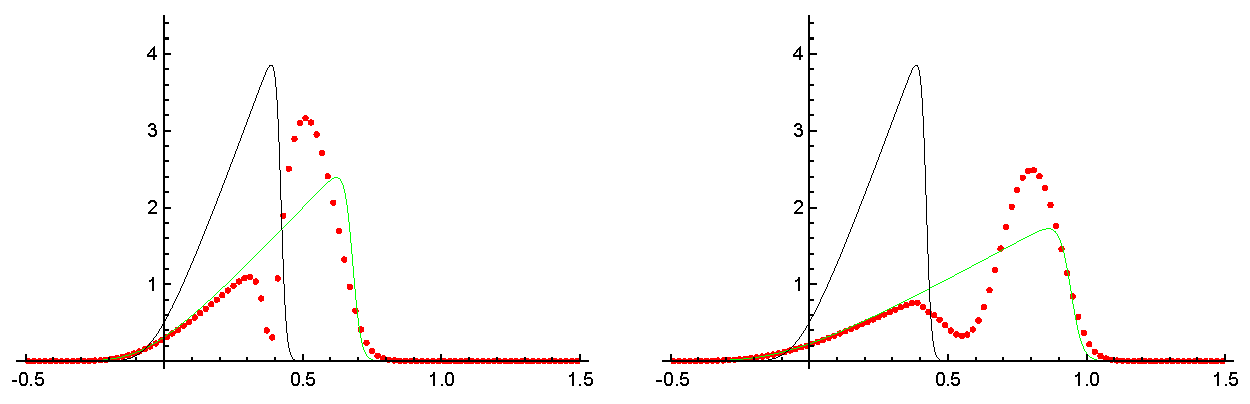
\includegraphics[width=\textwidth]{figures/tri100.pdf}
	\caption{Comparing the $\mathrm{IIOE}$ scheme with the exact triangular wave solution {\rm (\ref{triang})} in time $ t = 0.26 $ (left), $ t = 0.50 $ (right) for $ n=100 $, with $ \sigma=0.02 $,  $ \tau = 4h $.}
	\label{fig:triang-osc}
\end{figure}

\begin{figure}[h]
	\centering
	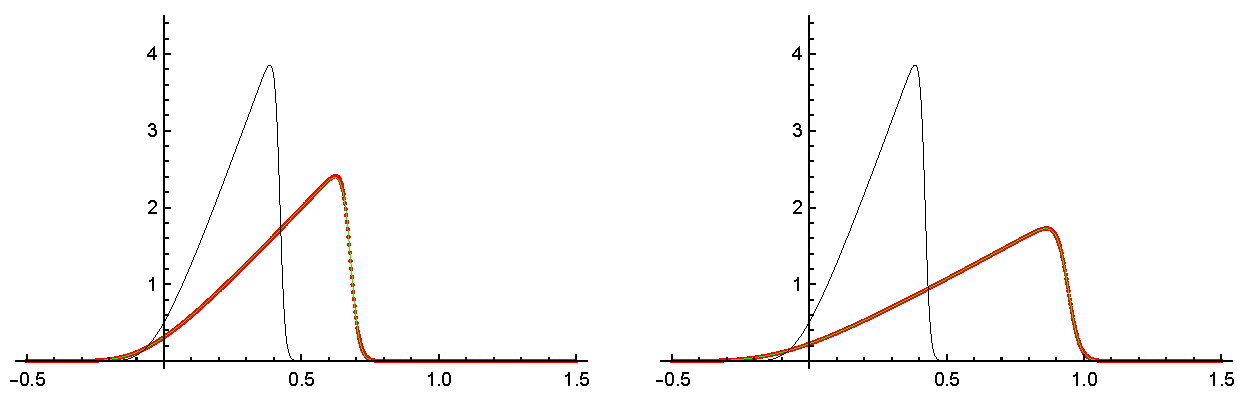
\includegraphics[width=\textwidth]{figures/tri800.pdf}
	\caption{Comparing the $\mathrm{IIOE}$ scheme with the exact triangular wave solution {\rm (\ref{triang})} in time $ t = 0.26 $ (left), $ t = 0.50 $ (right) for $ n=800 $ with $ \sigma=0.02 $,  $ \tau = 4h $.}
	\label{fig:triang}
\end{figure}

%====================================================================================================================================================

\textbf{Trigonometric solution.} Our last example is the trigonometric solution \eqref{trig} with $ a = 1.0025,\,b=1,\,\lambda = \pi^2 $ and $ \sigma = 0.01 $.
%\begin{equation}
%	u(x,t)=\frac{2\sigma b \pi \sin{\pi x}}{ae^{\sigma \pi^{2}t}+b\cos \pi x },
%\end{equation}
The errors are reported in Table \ref{ttrig}. A visual comparison of the numerical results with the exact solution is presented in Figure \ref{ftrig}.

\begin{table}[h!]
	\caption{Report on the $L_2$ errors of $\mathrm{IIOE}$ method for the trigonometric solution {\rm (\ref{trig})} of the viscous Burgers' equation {\rm (\ref{burg})} with $\sigma = 0.01$. }
	\begin{center} \footnotesize
		\begin{tabular}{|c|c|c|c|c|c|}
			\hline
			$n$ & $h$& $\tau$ & NTS & $L_2(I,L_2)$ & EOC\\
			\hline
			\lower.3ex\hbox{100} & \lower.3ex\hbox{0.02} & \lower.3ex\hbox{0.08} & \lower.3ex\hbox{15} & \lower.3ex\hbox{1.66 $10^{-2}$} &\\
			\hline
			\lower.3ex\hbox{200} & \lower.3ex\hbox{0.01} & \lower.3ex\hbox{0.04} & \lower.3ex\hbox{30} & \lower.3ex\hbox{3.18 $10^{-3}$} &\lower.3ex\hbox{2.38}\\
			\hline
			\lower.3ex\hbox{400} & \lower.3ex\hbox{0.005} & \lower.3ex\hbox{0.02} & \lower.3ex\hbox{60} & \lower.3ex\hbox{5.30 $10^{-4}$} &\lower.3ex\hbox{2.58}\\
			\hline
			\lower.3ex\hbox{800} & \lower.3ex\hbox{0.0025} & \lower.3ex\hbox{0.01} & \lower.3ex\hbox{120} & \lower.3ex\hbox{1.00 $10^{-4}$} &\lower.3ex\hbox{2.41}\\
			\hline
		\end{tabular}
	\end{center}
	\label{ttrig}
\end{table}

\begin{figure}[h!] 
	\centering
	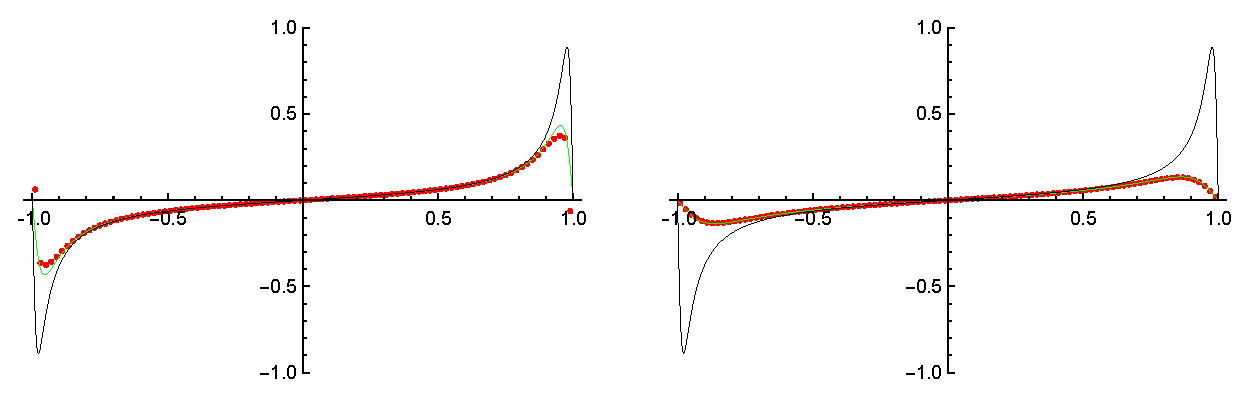
\includegraphics[width=\textwidth]{figures/trig100}
	\caption{Comparing the $\mathrm{IIOE}$ scheme with the exact trigonometric solution {\rm (\ref{trig})} in time $ t = 0.08 $ (left) and $ t = 0.96 $ (right) for $ n=100 $, with $ \sigma=0.01 $, $ b=1 $, $ a=1.0025 $, $ \tau = 4h $.}
	\label{ftrig} 
\end{figure} 

%====================================================================================================================================================
\newpage
\subsection{Numerical experiments - traffic flow}
In this section we solve the traffic flow equation \eqref{traffic} with $ v_{max} = 1 $.
As discussed earlier, by making certain assumptions about the flux function, we can transform the solutions of viscous Burgers' equation \eqref{burg} to obtain a solution for the density of the cars in the traffic flow problem (\ref{traffic}). Below we give an interpretation and comparison of the numerical and exact solutions of the traveling wave and the rarefaction wave solution in a traffic flow context. The experiments were presented in \cite{algoritmy}.

\textbf{Traveling wave.} A traveling wave can form in a traffic, when incoming cars are approaching a congestion or a line of cars staying behind a red light waiting for turning to green. In the congestion, the density $ \rho_r = 1 $, which means bumper to bumper traffic. The density of the incoming traffic was chosen to be $ \rho_l = 0.1 $, which means that there is one car/10 car lengths.

The exact solution of the density $ \rho $ was obtained as follows: considering the densities $ \rho_l = 0.1,\,\rho_r = 1 $ and using the relationship \eqref{u-ro} we can calculate $ u_l = 0.8$ and $ u_r = -1 $ for the traveling wave solution \eqref{travel} of the Burgers' equation. Then using the relationship (\ref{ro-u}) we obtain the solution for the density $ \rho $. This solution for the traffic density $ \rho $ was compared to the numerical solution using the IIOE scheme (\ref{iioe}). The errors are documented in Table \ref{tab:density_travel_sig1/1000}. The solution for $ D = 0.01 $ is presented in Figure \ref{fig:traffic_travel}.
\begin{table}[h!]
	\caption{Report on the $L_2$ errors of $\mathrm{IIOE}$ method for the traffic flow problem {\rm (\ref{traffic})} with $ D = 0.01$. }
	\begin{center} \footnotesize
		\begin{tabular}{|c|c|c|c|c|c|}
			\hline  
			$ n $ & $ h $ & $\tau$ & NTS & $L_2(I,L_2)$ & EOC\\
			\hline
			\lower.3ex\hbox{100} & \lower.3ex\hbox{0.01} & \lower.3ex\hbox{0.04} & \lower.3ex\hbox{12} & \lower.3ex\hbox{9.82 $10^{-4}$} &\\
			\hline
			\lower.3ex\hbox{200} & \lower.3ex\hbox{0.005} & \lower.3ex\hbox{0.02} & \lower.3ex\hbox{24} & \lower.3ex\hbox{2.36 $10^{-4}$} & \lower.3ex\hbox{2.05}\\
			\hline
			\lower.3ex\hbox{400} & \lower.3ex\hbox{0.0025} & \lower.3ex\hbox{0.01} & \lower.3ex\hbox{48} & \lower.3ex\hbox{5.94 $10^{-5}$} & \lower.3ex\hbox{1.99}\\
			\hline
			\lower.3ex\hbox{800} & \lower.3ex\hbox{0.00125} & \lower.3ex\hbox{0.005} & \lower.3ex\hbox{96} & \lower.3ex\hbox{1.53 $10^{-5}$} & \lower.3ex\hbox{1.96}\\
			\hline
		\end{tabular}
	\end{center}
	\label{tab:density_travel_sig1/1000}
\end{table}
\begin{figure}[h!]
	\centering
	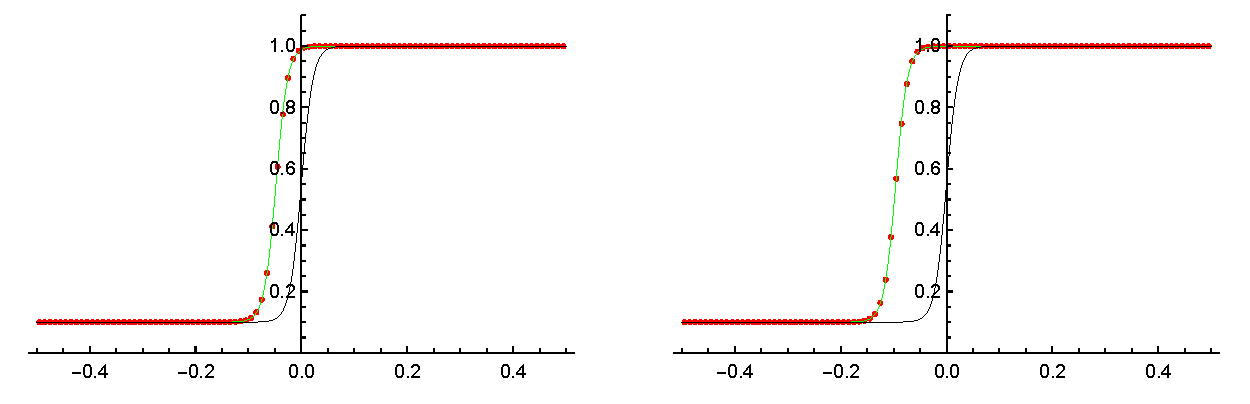
\includegraphics[width=.99\textwidth]{figures/travelTraffic_100_4h}
	\caption{Cars from left with traffic density $ \rho_l = 0.1 $ are approaching the congested region with $ \rho_r = 1 $. This would happen, for example, when cars are staying behind a red light. 
		The black line is the initial condition for the numerical computation, the red dots are the values computed by the IIOE scheme. The green line is the exact solution. The results of the numerical solution are shown at time $ t = 0.96 $, for $ n = 100 $, $ \tau = 4h $, $ D = 0.01 $.
	}
	\label{fig:traffic_travel}
\end{figure}

%====================================================================================================================================================
\newpage
\textbf{Rarefaction wave.} We also interpret the rarefaction wave solution in a traffic flow context. Imagine that the road is divided into two parts by the traffic light positioned at the origin. Cars to the left are staying behind the red light for $ t<0 $, so the density $ \rho_l = 1 $ there. On the right there is an empty road, $ \rho_r = 0 $. At time $ t = 0 $ the light turns green. This corresponds to the initial condition for a traffic light positioned at $ x = 0 $
\begin{equation}
\label{rare_traffic_init}
	\rho(0,x) =
	\begin{cases}
		1, &x\leq 0,\nonumber\\
		0, &x>0,\nonumber
	\end{cases}
\end{equation}
Right after the light turned green, the cars start to leave, the traffic rarefies. The exact solution for the density of equation  \ref{traffic}) was obtained in the same way as in our previous example. First, considering the values $ \rho_l = 1 $, $ \rho_r = 0 $ we calculate the corresponding values $ u_l = -1 $, $ u_r = 1 $ according to (\ref{u-ro}) for the rarefaction wave solution of the Burgers' equation. Then substituting the exact solution (\ref{rare}) to (\ref{ro-u}) we get the density function $ \rho $. Since the initial condition \eqref{rare_traffic_init} is discontinuous we started the computation at time $ t^0 = 0.01 $. The numerical solution for the density obtained by the IIOE scheme (\ref{iioe}) is presented for $ D = 0.01 $ in Figure ~\ref{fig:traffic_rare}. The errors are presented in Table ~\ref{tab:density_travel_rare}.
\begin{table}[h!]
	\caption{Report on the $L_2$ errors of $\mathrm{IIOE}$ method for the traffic flow problem {\rm (\ref{traffic})} with $ D = 0.01$. }
	\begin{center} \footnotesize
		\begin{tabular}{|c|c|c|c|c|c|}
			\hline  
			$ n $ & $ h $ & $\tau$ & NTS & $L_2(I,L_2)$ & EOC\\
			\hline
			\lower.3ex\hbox{100} & \lower.3ex\hbox{0.01} & \lower.3ex\hbox {0.04} & \lower.3ex\hbox{9} & \lower.3ex\hbox{2.49 $10^{-3}$} &\\
			\hline
			\lower.3ex\hbox{200} & \lower.3ex\hbox{0.005} & \lower.3ex\hbox{0.02} & \lower.3ex\hbox{18} & \lower.3ex\hbox{9.02 $10^{-4}$} & \lower.3ex\hbox{1.46}\\
			\hline
			\lower.3ex\hbox{400} & \lower.3ex\hbox{0.0025} & \lower.3ex\hbox{0.01} & \lower.3ex\hbox{36} & \lower.3ex\hbox{2.72 $10^{-4}$} & \lower.3ex\hbox{1.73}\\
			\hline
			\lower.3ex\hbox{800} & \lower.3ex\hbox{0.00125} & \lower.3ex\hbox{0.005} & \lower.3ex\hbox{72} & \lower.3ex\hbox{7.62 $10^{-5}$} & \lower.3ex\hbox{1.84}\\
			\hline
		\end{tabular}
	\end{center}
	\label{tab:density_travel_rare}
\end{table}
\begin{figure}[h!]
	\centering
	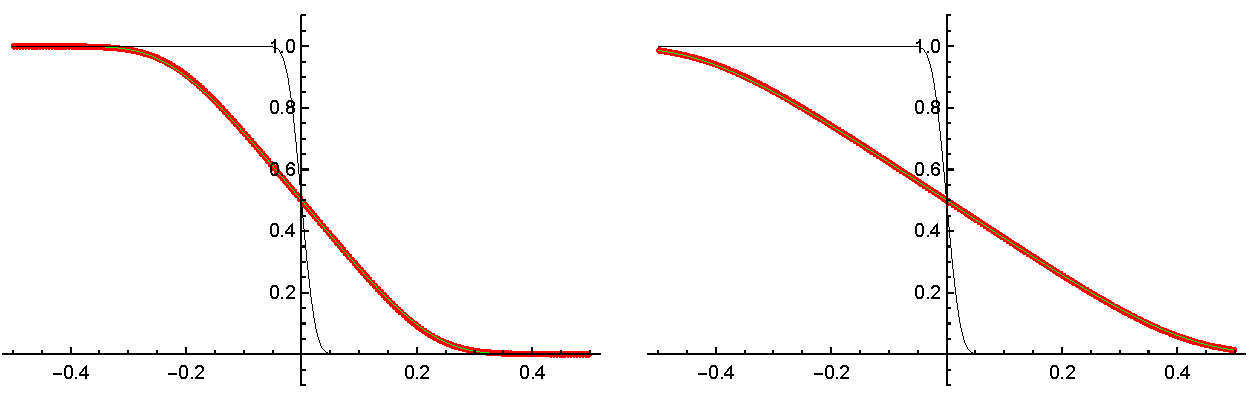
\includegraphics[width=.99\textwidth]{figures/traffic_Rare_200_4h}
	\caption{At $ t<0 $ cars to the left of the origin are staying behind a red light, the density $ \rho_l = 1 $. To the right there is an empty road, $ \rho_r = 0 $. At time $ t = 0 $ the traffic light at the origin turns green and cars start to leave. The exact solution(black) is compared with the numerical solution obtained by the IIOE scheme \eqref{iioe}(red) at time $ t = 0.18 $(left) and $ t = 0.36 $(right) for $ n = 200 $, $ \tau = 4h $, $ D = 0.01 $.The initial condition at time $ t^0 = 0.01 $ is given in black.}
	\label{fig:traffic_rare}
\end{figure}
%====================================================================================================================================================
\newpage
\section{Scalar conservation laws}
Let us consider the scalar conservation law of the form
\begin{equation}
	u_t + f(u)_x = 0,
	\label{scalar_conservation}
\end{equation}
where $ u = u(t, x) $ is the unknown scalar quantity, $ f(u) $ is a flux function. We can equivalently write the equation in quasi-linear or advective form \cite{lev, whitham} as
\begin{equation}
	u_t + f'(u)u_x = 0
	\label{quasi-linear}
\end{equation}
where $ f'(u) $ is the characteristic speed.\\
The equation
\begin{equation}
	\label{advection_constant}
	u_t + vu_x = 0,
\end{equation}
is the simplest scalar conservation law with the flux function $ f(u) = vu $ with constant characteristic speed $ f'(u) = v $. Considering positive characteristic speed $ v > 0 $, the IIOE scheme \eqref{iioe0} can be written as
\begin{equation}
	\label{adv_cons_v+}
	u_i^{n} = u_i^{n - 1} - \frac{\tau}{h}\left((vu^n_{i} + vu^{n-1}_{i+1}) - (v u^n_{i-1} + v u^{n-1}_{i})\right).
\end{equation}
Similarly, for $ v < 0 $ the scheme \eqref{iioe0} reads
\begin{equation}
	\label{adv_cons_v-}
	u_i^{n} = u_i^{n - 1} - \frac{\tau}{h}\left[(vu^n_{i} + vu^{n-1}_{i-1}) - (v u^n_{i+1} + v u^{n-1}_{i})\right].
\end{equation}
Notice that both \eqref{adv_cons_v+} and \eqref{adv_cons_v-} have the form of a conservative finite volume scheme \eqref{finite_volume}, if we define the numerical flux as
\begin{equation}
	\label{iioe_lin_adv_flux}
	F_{i - 1/2} =
\begin{cases}
	\dfrac{1}{2}\left(vu^n_{i-1} + vu^{n-1}_{i}\right) &  \text{if } v > 0\\
	\\
	\dfrac{1}{2}\left(vu^n_{i} + vu^{n-1}_{i-1}\right) &  \text{if } v < 0.
\end{cases}
\end{equation}
Based on this observation, we suggest that for scalar conservation laws \eqref{scalar_conservation} we should write the IIOE scheme as a conservative finite volume method \eqref{finite_volume} with numerical flux depending on the sign characteristic speed $ f'(u) $. We denote $ f_i^n:= f(u_i^n) $, then the average flux is defined by
\begin{equation}
	F_{i - 1/2} = 
\begin{cases}
	\label{flux_iioe}
	\dfrac{1}{2}\left(f^n_{i-1} + f^{n-1}_{i}\right) &  \text{if } f'(u)\big|_{\substack{x_{i-1/2}}} > 0\\
	\\
	\dfrac{1}{2}\left(f^{n-1}_{i-1} + f^{n}_{i}\right) &  \text{if } f'(u)\big|_{\substack{x_{i-1/2}}} < 0,
\end{cases}
\end{equation}
where we calculate the characteristic speed at a given interface from the previous time step $ n-1 $, i.e.\
\begin{equation}
	\label{iioe_char_speed}
	f'(u)\big|_{\substack{x_{i-1/2}}} = \frac{f'(u_{i-1}^{n-1}) + f'(u_{i}^{n-1})}{2}.
\end{equation}
It should be noted that \eqref{adv_cons_v+}, \eqref{adv_cons_v-} was already recognized in \cite{iioe2012, iioe2}.

If we consider the nonlinear transport equation
\begin{equation}
	u_t + \left(\frac{u^2}{2}\right)_x = 0, 
	\label{inviscid}
\end{equation}
with flux given by $ f(u) = u^2/2 $ and characteristic speed $ f'(u) = u $, which is known as the inviscid Burgers' equation, since it is \eqref{burg} with zero viscosity $ \sigma = 0 $, the numerical flux at cell interfaces is defined by
\begin{equation}
	\label{basic_iioe_burgers_flux}
	F_{i - 1/2} = 
\begin{cases}
	\dfrac{1}{2}\left[\dfrac{(u^n_{i-1})^2}{2} + \dfrac{(u^{n-1}_{i})^2}{2} \right] &  \text{if } u_{i-1/2} > 0\\
	\\
\dfrac{1}{2}\left[\dfrac{(u^n_{i})^2}{2} + \dfrac{(u^{n-1}_{i-1})^2}{2} \right] &  \text{if } u_{i-1/2} < 0
\end{cases}
\end{equation}
where $ u_{i-1/2} = (u_{i-1}^{n-1} + u_{i}^{n-1})/2 $. Numerical experiments for the inviscid Burgers' equation will be presented in sections 2.4.2 and 2.5.2.
\par \textbf{Remark.} For nonlinear conservation laws, where the solutions can develop shocks, it is important that the numerical scheme is conservative, i.e.\ it can be written in the form of \eqref{finite_volume}. The Lax-Wendroff theorem tells us, that if this holds, the numerical solution of a stable method converges to a weak solution of the differential equation \eqref{scalar_conservation}, as the grid is refined. To ensure that the weak solution is a physically relevant one, the numerical scheme must also satisfy an entropy condition \cite{lev}.
%For convenience, we show that the scheme is identical to the IIOE scheme presented in previous works, in which the scheme was derived using the quasi-linear or advective form \eqref{quasi-linear} as in \cite{iioe0, algoritmy}. For simplicity, we assume that $ f'(u) = u > 0 $. Then we write the scheme in terms of fluxes as\[u_i^{n} = u_i^{n - 1} - \frac{\tau}{h}\Bigg[\underbrace{\frac{1}{2}\left(\frac{(u^n_{i})^2}{2} + \frac{(u^{n-1}_{i+1})^2}{2} \right)}_{F_{i + 1/2}}- \underbrace{\frac{1}{2}\left(\frac{(u^n_{i-1})^2}{2} + \frac{(u^{n-1}_{i})^2}{2}\right)}_{F_{i - 1/2}}\Bigg].\]After simplifying we get\[u_i^{n} = u_i^{n - 1} - \dfrac{\tau}{4h}\left[(u^n_{i})^2 + (u^{n-1}_{i+1})^2 - (u^n_{i-1})^2 - (u^{n-1}_{i})^2\right].\]Putting the unknown values at time step $ n $ to the left hand side we get\begin{equation}	u_i^{n} + \dfrac{\tau}{4h}\left[(u^n_{i})^2 - (u^n_{i-1})^2\right] = 	u_i^{n - 1} + \dfrac{\tau}{4h}\left[(u^{n-1}_{i})^2 - (u^{n-1}_{i+1})^2\right].	\label{inviscid_0}\end{equation}Now we show that this is equivalent to the scheme \eqref{iioe0}.The time dependent inflow and outflow coefficients are\begin{eqnarray}	a^{in,n}_{i-1/2} = \textrm{max}(v^{n}_{i-1/2},0),\quad 	a^{out,n}_{i-1/2} = \textrm{min}(v^{n}_{i-1/2},0), \nonumber	\\	a^{in,n}_{i+1/2} = \textrm{max}(-v^{n}_{i+1/2},0),\quad 	a^{out,n}_{i+1/2} = \textrm{min}(-v^{n}_{i+1/2},0) \nonumber\end{eqnarray}with velocities at the interfaces\[ v^{n}_{i-1/2} = \dfrac{u^{n}_i + u^{n}_{i-1}}{2},\quadv^{n}_{i+1/2} = \dfrac{u^{n}_i + u^{n}_{i+1}}{2}.\]Assuming $ f'(u) = u > 0 $ we get\[a^{in,n}_{i-1/2} = \dfrac{u^{n}_i + u^{n}_{i-1}}{2},\quad a^{out,n}_{i-1/2} = 0,\quad a^{in,n}_{i + 1/2} = 0,\quad a^{out,n}_{i+1/2} = -\dfrac{u^{n}_i + u^{n}_{i+1}}{2}.\]Substituting into the numerical scheme and assuming $ \sigma = 0 $ we end up with\begin{equation}	u^n_i + \frac{\tau}{2h} \dfrac{u^{n}_i + u^{n}_{i-1}}{2} \left(u^n_i - u^n_{i-1}\right)	= 	u^{n-1}_i - \frac{\tau}{2h} 	\left(-\dfrac{u^{n-1}_i + u^{n-1}_{i+1}}{2}\right) \left(u^{n-1}_i - u^{n-1}_{i+1}\right)\end{equation}after simplifying we get\begin{equation}	\label{inviscid_1}	u_i^{n} + \dfrac{\tau}{4h}\left[(u^n_{i})^2 - (u^n_{i-1})^2\right] = 	u_i^{n - 1} + \dfrac{\tau}{4h}\left[(u^{n-1}_{i})^2 - (u^{n-1}_{i+1})^2\right]\end{equation}which coincides with (\ref{inviscid_0}) derived previously.
%====================================================================================================================================================\textbf{Traffic flow}. For the LWR model described earlier we have flux $ f(\rho) = \rho (1 - \rho) $ with characteristic speed $ f'(\rho) = 1 - 2\rho $. The numerical flux at the interface is then\[F_{i - 1/2} =\begin{cases}	\dfrac{1}{2}\left[\rho^n_{i-1} (1 - \rho^n_{i-1}) + \rho^{n-1}_{i} (1 - \rho^{n-1}_{i}) \right] &  \text{if } (1-2\rho_{i-1/2}) > 0\\	\\	\dfrac{1}{2}\left[\rho^n_{i} (1 - \rho^n_{i}) + \rho^{n-1}_{i-1} (1 - \rho^{n-1}_{i-1}) \right] &  \text{if } (1-2\rho_{i-1/2}) < 0,\end{cases}\]where again, the characteristic speed is calculated using the IIOE approach.\\Now let us compare with our previously derived IIOE scheme. Again, we will consider only the case if $ f'(\rho) = 1 - 2\rho > 0 $. Substituting the numerical fluxes the scheme becomes\[\rho_i^{n} = \rho_i^{n - 1} - \dfrac{\tau}{h}\Bigg(\underbrace{\frac{1}{2}\left[\rho^n_{i} (1 - \rho^n_{i}) + \rho^{n-1}_{i+1} (1 - \rho^{n-1}_{i+1}) \right]}_{F_{i + 1/2}}- \underbrace{\frac{1}{2}\left[\rho^n_{i-1} (1 - \rho^n_{i-1}) + \rho^{n-1}_{i} (1 - \rho^{n-1}_{i}) \right]}_{F_{i - 1/2}}\Bigg).\]After simplifying and putting the unknown values at time step $ n $ to the left hand side we get\[\rho_i^{n} + \frac{\tau}{2h}\left[\rho^n_{i} (1 - \rho^n_{i}) - \rho^n_{i-1} (1 - \rho^n_{i-1})\right]=\rho_i^{n - 1} - \dfrac{\tau}{2h}\left[\rho^{n-1}_{i+1} (1 - \rho^{n-1}_{i+1}) - \rho^{n-1}_{i} (1 - \rho^{n-1}_{i})\right].\]Multiplying the terms in the parentheses we end up with\begin{equation}	\label{traffic_fromflux}	\rho_i^{n} + \frac{\tau}{2h}\left(\rho^n_{i} - (\rho^n_{i})^2 - \rho^n_{i-1} + (\rho^n_{i-1})^2\right)=\rho_i^{n - 1} - \dfrac{\tau}{2h}\left[\rho^{n-1}_{i+1} - (\rho^{n-1}_{i+1})^2 - \rho^{n-1}_{i} + (\rho^{n-1}_{i})^2\right].\end{equation}Now we would like to show that we end up with the same scheme also with the different approach as in \cite{algoritmy}.\\In this case we calculate the velocities at the interfaces as\[v^{n}_{i-1/2} = 1 - 2\rho^n_{i-1/2},\quadv^{n}_{i+1/2} = 1 - 2\rho^n_{i+1/2}.\]The densities at the interfaces we calculate as $ \rho^n_{i-1/2} = (\rho^n_{i-1} + \rho^n_{i})/2 $ and $ \rho^n_{i+1/2} = (\rho^n_{i} + \rho^n_{i+1})/2 $, similarly as in \cite{algoritmy}. The inflow and outflow coefficients, considering that $ f'(\rho) = 1 - 2\rho > 0 $ and cancelling common factors become\[a^{in,n}_{i-1/2} = 1 - \left(\rho^n_{i-1} + \rho^n_{i}\right),\quad a^{out,n}_{i-1/2} = 0,\quad a^{in,n}_{i + 1/2} = 0 \text{ and } a^{out,n}_{i+1/2} = -\left(1 - \left(\rho^n_{i} + \rho^n_{i+1}\right) \right).\]Substituting into the scheme \eqref{iioe0}, changing $ u_i^n $ to $ \rho_i^n $. we get\[\rho^n_i + \frac{\tau}{2h} \left[1 - (\rho^n_{i-1} + \rho^n_{i})\right] \left(\rho^n_i - \rho^n_{i-1}\right)= \rho^{n-1}_i - \frac{\tau}{2h} \left[-\left(1 - (\rho^{n-1}_{i} + \rho^{n-1}_{i+1}) \right)\right] \left(\rho^{n-1}_i - \rho^{n-1}_{i+1}\right)\]Multiplying the terms in the parentheses we end up with\[\rho^n_i + \frac{\tau}{2h} \left[\rho^n_i - \rho^n_{i-1} - (\rho^n_{i})^2 + (\rho^n_{i-1})^2\right] = \rho^{n-1}_i - \frac{\tau}{2h} \left[-\rho^{n-1}_i + \rho^{n-1}_{i+1} + (\rho^{n-1}_{i})^2 - (\rho^{n-1}_{i+1})^2\right] \]which agrees with the scheme \eqref{traffic_fromflux} derived previously.
%====================================================================================================================================================
\subsection{Formal second order consistency}

\begin{theorem}
	For scalar conservation laws \eqref{scalar_conservation} the IIOE scheme with numerical fluxes at the interfaces defined by \eqref{flux_iioe} is formally second order for smooth solutions on a uniform grid and the consistency error is of order $\mathcal{O}(h^2) + \mathcal{O}(\tau h) + \mathcal{O}(\tau^2)$.
\end{theorem}
\begin{proof}
	 Let us consider, that $ u^n_i := u(t^n, x_i) $ is a solution of \eqref{scalar_conservation} and $ f^n_i := f(u(t^n, x_i)) $ in the scheme \eqref{flux_iioe}. The characteristic speed at the interfaces is calculated according to \eqref{iioe_char_speed} from the previous time step. As the numerical fluxes, thus the scheme, depend on the sign of the characteristic speed at the interfaces, we have to distinguish four cases:\\
\textbf{Case 1: }$ f'(u)\big|_{\substack{x_{i-1/2}}},\,f'(u)\big|_{\substack{x_{i+1/2}}} > 0 $. In that case the IIOE scheme reads
\[
\frac{u_i^{n} - u_i^{n - 1}}{\tau} = - \frac{1}{2h}\left[(f_i^n + f_{i+1}^{n-1}) - (f_{i-1}^n + f_i^{n-1})\right].
\]
The Taylor expansion of $ u $ in time yields
\[
u_i^n = u_i^{n-1} + \tau \partial_t u_i^{n-1} + \frac{\tau^2}{2}\partial_t^2 u_i^{n-1} + \mathcal{O}(\tau^3),\quad
u_i^{n-1} = u_i^{n} - \tau \partial_t u_i^n + \frac{\tau^2}{2}\partial_t^2 u_i^n + \mathcal{O}(\tau^3).
\]
Subtracting these two expressions we get
\begin{equation}
	u_i^n - u_i^{n-1} = \frac{\tau}{2}\left(\partial_t u_i^{n-1} + \partial_t u_i^n\right) + 
	\underbrace{\frac{\tau^2}{4}\left(\partial_t^2 u_i^{n-1} - \partial_t^2 u_i^n\right)}_{\mathcal{O}(\tau^3)}
	+ \mathcal{O}(\tau^3).
	\label{u_i^n - u_i^{n-1}}
\end{equation}
The Taylor expansion of $ f $ in space yields
\begin{equation}
	f_{i-1}^n = f_i^n - h\partial_x f_i^n + \frac{h^2}{2}\partial_x^2 f_i^n + \mathcal{O}(h^3) = f_i^n + h\partial_t u_i^n + \frac{h^2}{2}\partial_x^2 f_i^n + \mathcal{O}(h^3),
	\label{f_{i-1}^n}
\end{equation}
\begin{equation}
	f_{i+1}^{n-1} = f_i^{n-1} + h \partial_x f_i^{n-1} + \frac{h^2}{2} \partial_x^2 f_i^{n-1} + \mathcal{O}(h^3) = 
	f_i^{n-1} - h \partial_t u_i^{n-1} + \frac{h^2}{2} \partial_x^2 f_i^{n-1} + \mathcal{O}(h^3).
	\label{f_{i+1}^{n-1}}
\end{equation}
In both cases we used the relationship between partial derivatives $ \partial_t u = \partial_x f $, assuming that the differential equation holds.
Now we subtract \eqref{f_{i+1}^{n-1}} from \eqref{f_{i-1}^n} to get
\[
f_{i+1}^{n-1} - f_{i-1}^n = f_i^{n-1} - f_i^n - h\left(\partial_t u_i^{n-1} + \partial_t u_i^{n}\right)
+ \underbrace{\frac{h^2}{2} \left(\partial_x^2 f_i^{n-1} - \partial_x^2 f_i^{n}\right)}_{\mathcal{O}(h^2\tau)} + \mathcal{O}(h^3).
\]
Multiplying both sides by $ \tau/(2h) $ and by algebraic manipulation we get
\begin{equation}
	\frac{\tau}{2}\left(\partial_t u_i^{n-1} + \partial_t u_i^{n}\right) = - \frac{\tau}{2h}\left[(f_i^n + f_{i+1}^{n-1}) - (f_{i-1}^n + f_i^{n-1})\right] + \mathcal{O}(h\tau^2) + \mathcal{O}(h^2\tau).
	\label{tau2}
\end{equation}
Substituting \eqref{tau2} to \eqref{u_i^n - u_i^{n-1}} we get
\[	u_i^n - u_i^{n-1} = - \frac{\tau}{2h}\left[(f_i^n + f_{i+1}^{n-1}) - (f_{i-1}^n + f_i^{n-1})\right] + \mathcal{O}(h\tau^2) + \mathcal{O}(h^2\tau) + \mathcal{O}(\tau^3),\]
where we can recognize the IIOE scheme. Dividing by $ \tau $ we get the consistency error
\begin{equation}
	\frac{u_i^n - u_i^{n-1}}{\tau} = - \frac{1}{2h}\left[(f_i^n + f_{i+1}^{n-1}) - (f_{i-1}^n + f_i^{n-1})\right] + \mathcal{O}(h\tau) + \mathcal{O}(h^2) + \mathcal{O}(\tau^2).
\end{equation}
\textbf{Case 2: }$ f'(u)\big|_{\substack{x_{i-1/2}}},\,f'(u)\big|_{\substack{x_{i+1/2}}} \leq 0 $, the IIOE scheme then reads
\[
\frac{u_i^{n} - u_i^{n - 1}}{\tau} = - \frac{1}{2h}\left[(f_i^{n-1} + f_{i+1}^{n}) - (f_{i-1}^{n-1} + f_i^{n})\right].
\]
The Taylor expansion of $ f $ in space yields
\begin{equation}
	f_{i-1}^{n-1} = f_{i}^{n-1} - h\partial_x f_{i}^{n-1} + \frac{h^2}{2}\partial_x^2 f_{i}^{n-1} + \mathcal{O}(h^3) = f_{i}^{n-1} + h\partial_t u_{i}^{n-1} + \frac{h^2}{2}\partial_x^2 f_i^{n-1} + \mathcal{O}(h^3),
	\label{f_{i-1}^{n-1}}
\end{equation}
\begin{equation}
	f_{i+1}^{n} = f_i^{n} + h \partial_x f_i^{n} + \frac{h^2}{2} \partial_x^2 f_i^{n} + \mathcal{O}(h^3) = 
	f_i^{n} - h \partial_t u_i^{n} + \frac{h^2}{2} \partial_x^2 f_i^{n} + \mathcal{O}(h^3).
	\label{f_{i+1}^{n}}
\end{equation}
Now we subtract \eqref{f_{i-1}^{n-1}} from \eqref{f_{i+1}^{n}} to get
\[
f_{i+1}^{n} - f_{i-1}^{n-1} = f_i^{n} - f_{i}^{n-1} - h(\partial_t u_i^{n} + \partial_t u_{i}^{n-1}) + \underbrace{\frac{h^2}{2} \left(\partial_x^2 f_i^{n} - \partial_x^2 f_i^{n-1}\right)}_{\mathcal{O}(h^2\tau)} + \mathcal{O}(h^3).
\]
Multiplying both sides by $ \tau/(2h) $ and by algebraic manipulation we get
\begin{equation}
	\frac{\tau}{2}\left(\partial_t u_i^{n} + \partial_t u_i^{n-1}\right) = - \frac{\tau}{2h}\left[(f_i^{n-1} + f_{i+1}^{n}) - (f_{i-1}^{n-1} + f_i^{n})\right] + \mathcal{O}(h\tau^2) + \mathcal{O}(h^2\tau).
	\label{tau2_1}
\end{equation}
Substituting \eqref{tau2_1} to \eqref{u_i^n - u_i^{n-1}} we get
\[	u_i^n - u_i^{n-1} = - \frac{\tau}{2h}\left[(f_i^{n-1} + f_{i+1}^{n}) - (f_{i-1}^{n-1} + f_i^{n})\right] + \mathcal{O}(h\tau^2) + \mathcal{O}(h^2\tau) + \mathcal{O}(\tau^3),\]
where we can recognize the IIOE scheme. Dividing by $ \tau $ we get the consistency error
\begin{equation}
	\frac{u_i^n - u_i^{n-1}}{\tau} = - \frac{1}{2h}\left[(f_i^{n-1} + f_{i+1}^{n}) - (f_{i-1}^{n-1} + f_i^{n})\right] + \mathcal{O}(h\tau) + \mathcal{O}(h^2) + \mathcal{O}(\tau^2).
\end{equation}
Two other cases remain, when the characteristic speed has different sign at the interfaces.\\
\textbf{Case 3: } $ f'(u)\big|_{\substack{x_{i-1/2}}} < 0,  \,f'(u)\big|_{\substack{x_{i+1/2}}} > 0 $, for which the scheme reads
\[
\frac{u_i^{n} - u_i^{n - 1}}{\tau} = - \frac{1}{2h}\left[(f_i^{n} + f_{i+1}^{n-1}) - (f_{i-1}^{n-1} + f_i^{n})\right],
\]
which reduces to
\begin{equation}
	\label{Taylor_exp}
	\frac{u_i^{n} - u_i^{n - 1}}{\tau} = - \frac{f_{i+1}^{n-1} - f_{i-1}^{n-1}}{2h},
\end{equation}
where we can recognize a centered difference for the spatial derivative of the flux function. By Taylor expansion in space of $ f $ at time step $ n-1 $ we get
\begin{align}
	f_{i+1}^{n-1} &= f_i^{n-1} + h \partial_x f_i^{n-1} + \frac{h^2}{2} \partial_x^2 f_i^{n-1} + \mathcal{O}(h^3) = 
	f_i^{n-1} - h \partial_t u_i^{n-1} + \frac{h^2}{2} \partial_x^2 f_i^{n-1} + \mathcal{O}(h^3),\nonumber\\
	f_{i-1}^{n-1} &= f_i^{n-1} - h\partial_x f_i^{n-1} + \frac{h^2}{2}\partial_x^2 f_i^{n-1} + \mathcal{O}(h^3) = f_i^{n-1} + h\partial_t u_i^{n-1} + \frac{h^2}{2}\partial_x^2 f_i^{n-1} + \mathcal{O}(h^3)\nonumber.
\end{align}
After subtraction and dividing by $ (-2h) $ we get
\begin{equation}
	\label{fderout}
	-\frac{f_{i+1}^{n-1} - f_{i-1}^{n-1}}{2h} = \partial_t u_i^{n-1} + \mathcal{O}(h^2).
\end{equation}
By Taylor expansion of $ u $ in time we get
\begin{equation}
	u_i^n = u_i^{n-1} + \tau \partial_t u_i^{n-1} + \frac{\tau^2}{2}\partial_t^2 u_i^{n-1} + \mathcal{O}(\tau^3).
\end{equation}
By rearranging terms and dividing by $ \tau $ we get
\begin{equation}
	\frac{u_i^{n} -  u_i^{n-1}}{\tau} = \partial_t u_i^{n-1} + \frac{\tau}{2}\partial_t^2 u_i^{n-1} + \mathcal{O}(\tau^2).
\end{equation}
Substituting \eqref{fderout} we end up with
\begin{equation}
	\label{Taylor_out_scheme}
	\frac{u_i^{n} -  u_i^{n-1}}{\tau} = -\frac{f_{i+1}^{n-1} - f_{i-1}^{n-1}}{2h} + \frac{\tau}{2}\partial_t^2 u_i^{n-1} + \mathcal{O}(\tau^2) + \mathcal{O}(h^2).
\end{equation}
We want to show that the term $ \frac{\tau}{2}\partial_t^2 u_i^{n-1} $ is $ \mathcal{O}(\tau h) $. From the conservation law \eqref{scalar_conservation} we know that $ \partial_t u_i^{n-1} = -\partial_x f(u_i^{n-1}) = - f'(u_i^{n-1}) \partial_x u_i^{n-1} $. Then
\begin{align}
	\partial^2_t u_i^{n-1} = - \partial_t \left(f'(u_i^{n-1}) \partial_x u_i^{n-1}\right) &=
	- f''(u_i^{n-1}) \underbrace{\partial_t u_i^{n-1}}_{=- f'(u_i^{n-1}) \partial_x u_i^{n-1}} \partial_x u_i^{n-1} - f'(u_i^{n-1}) \partial_t \partial_x u_i^{n-1}=\nonumber\\
	&= f'(u_i^{n-1}) \left(f''(u_i^{n-1}) (\partial_x u_i^{n-1})^2 - \partial_t \partial_x u_i^{n-1}\right),
\end{align}
where we took out the common factor $ f'(u_i^{n-1}) $. Now, similarly as in \cite{iioe2012, iioe2}, we want to use the fact that the characteristic speed changes sign inside the cell. If $ f'(u) $ is smooth and $ f'(u)\big|_{\substack{x_{i-1/2}}} < 0,  \,f'(u)\big|_{\substack{x_{i+1/2}}} > 0 $ then there exists some $ x_* \in (x_{i-1/2}, x_{i+1/2}) $ for which $ f'(u)\big|_{\substack{x_{*}}} = 0 $. In that case both fluxes represent outflows so we calculate them in the previous time step $ n-1 $. From the Taylor expansion of the speed around $ x_* $ we get
\[
f'(u_i^{n-1}) = \underbrace{f'(u_*^{n-1})}_{=0} + \underbrace{(x_i - x_*)}_{\mathcal{O}(h)}\partial_x f'(u_*^{n-1}) + \mathcal{O}(h^2),
\]
from which we see that $ \partial_t^2 u_i^{n-1} $ is $ \mathcal{O}(h) $ so the term $ \frac{\tau}{2}\partial_t^2 u_i^{n-1} $ in \eqref{Taylor_out_scheme} is $ \mathcal{O}(\tau h) $.\\
\textbf{Case 4: }The last possible case is when $ f'(u)\big|_{\substack{x_{i-1/2}}} > 0,  \,f'(u)\big|_{\substack{x_{i+1/2}}} < 0 $, for which we have
\[
\frac{u_i^{n} - u_i^{n - 1}}{\tau} = - \frac{1}{2h}\left[(f_i^{n-1} + f_{i+1}^{n}) - (f_{i-1}^{n} + f_i^{n-1})\right],
\]
which simplifies to
\[
\frac{u_i^{n} - u_i^{n - 1}}{\tau} = - \frac{f_{i+1}^{n} - f_{i-1}^{n}}{2h},
\]
where similarly as in the previous case, we can recognize a centered difference for the flux function on the right hand side calculated at time step $ n $. The derivation is almost the same as for \textbf{Case 3}.
We need the following Taylor expansions of $ f $
\begin{align}
	f_{i+1}^{n} &= f_i^{n} + h \partial_x f_i^{n} + \frac{h^2}{2} \partial_x^2 f_i^{n} + \mathcal{O}(h^3) = 
	f_i^{n} - h \partial_t u_i^{n} + \frac{h^2}{2} \partial_x^2 f_i^{n} + \mathcal{O}(h^3),\label{fin_1}\\
	f_{i-1}^n &= f_i^n - h\partial_x f_i^n + \frac{h^2}{2}\partial_x^2 f_i^n + \mathcal{O}(h^3) = f_i^n + h\partial_t u_i^n + \frac{h^2}{2}\partial_x^2 f_i^n + \mathcal{O}(h^3).
	\label{fin_2}
\end{align}
Subtracting \eqref{fin_2} from \eqref{fin_1} and dividing by $ (-2h) $ we get
\begin{equation}
	\label{fderin}
	-\frac{f_{i+1}^{n} - f_{i-1}^n}{2h} = \partial_t u_i^{n} + \mathcal{O}(h^2).
\end{equation}
We need the Taylor expansion of $ u $
\begin{equation}
	u_i^{n-1} = u_i^{n} - \tau \partial_t u_i^n + \frac{\tau^2}{2}\partial_t^2 u_i^n + \mathcal{O}(\tau^3).
	\label{uin}
\end{equation}
By rearranging terms and dividing by $ \tau $ we get
\begin{equation}
	\frac{u_i^{n} -  u_i^{n-1}}{\tau} = \partial_t u_i^n + \frac{\tau}{2}\partial_t^2 u_i^n + \mathcal{O}(\tau^2).
\end{equation}
Substituting \eqref{fderin} we end up with
\begin{equation}
	\label{Taylor_im_scheme}
	\frac{u_i^{n} -  u_i^{n-1}}{\tau} = -\frac{f_{i+1}^{n} - f_{i-1}^n}{2h} + \frac{\tau}{2}\partial_t^2 u_i^n + \mathcal{O}(\tau^2) + \mathcal{O}(h^2).
\end{equation}
It remains to show that the term $ \frac{\tau}{2}\partial_t^2 u_i^n $ is $ \mathcal{O}(\tau h) $. We use the notation $ f'(u(t^n, x_i)) = f'(u_i^n) $. From the conservation law \eqref{scalar_conservation} we know that $ \partial_t u_i^n = -\partial_x f(u_i^n) = - f'(u_i^n) \partial_x u_i^n $. Then
\begin{align}
	\partial^2_t u_i^n = - \partial_t \left(f'(u_i^n) \partial_x u_i^n\right) &=
	- f''(u_i^n) \underbrace{\partial_t u_i^n}_{=- f'(u_i^n) \partial_x u_i^n} \partial_x u_i^n - f'(u_i^n) \partial_t \partial_x u_i^n=\nonumber\\
	&= f'(u_i^n) \left(f''(u_i^n) (\partial_x u_i^n)^2 - \partial_t \partial_x u_i^n\right),
\end{align}
where we took out the common factor $ f'(u_i^n) $. As before, we use the fact that the characteristic speed changes sign inside the cell. We assume, that $ f'(u) $ is smooth in space and time, then $ f'(u_i^{n}) = f'(u_i^{n-1}) + \mathcal{O}(\tau) $. We have already shown, that $ f'(u_i^{n-1}) $ is of order $ \mathcal{O}(h) $, from which we see that $ \partial_t^2 u_i^n $ is $ \mathcal{O}(h) + \mathcal{O}(\tau) $ so the term $ \frac{\tau}{2}\partial_t^2 u_i^n $ in \eqref{Taylor_im_scheme} is $ \mathcal{O}(\tau h) + \mathcal{O}(\tau^2) $.
\end{proof}
%====================================================================================================================================================
\subsection{Numerical experiments}
In order to have some evidence that the IIOE scheme with numerical fluxes defined by \eqref{flux_iioe} is second order accurate for smooth solutions of conservation laws of the form \eqref{scalar_conservation}, we performed numerical experiments for solutions of the advection equation with constant speed \eqref{advection_constant} and nonlinear transport equation \eqref{inviscid}. In both cases, an exact Dirichlet boundary condition is given at the inflow endpoint.

\textbf{Advection with constant speed.} First we chose a solution of the advection equation \eqref{advection_constant} with $ v = 1 $ and initial condition given by
\begin{equation}
	\label{lin_adv_smooth_0}
	u^0(x) = 1+\frac{1}{2}\left(1- \tanh \left(\frac{x + 0.5}{0.2}\right)\right).
\end{equation}
The exact solution is given by
\[
u(t, x) = u^0(x - t).
\]
The numerical solution was obtained by the IIOE scheme with numerical flux defined by \eqref{adv_cons_v+}. The computation was performed on a space interval (-1,1) and time interval (0, 1). The results are reported in Table ~\ref{tab:iioe_smooth_const}. A visual comparison of the numerical solution with the exact one can be seen in Figure ~\ref{fig:basic_iioe_advection}.
\begin{table}[ht]
	\caption{Report on the $L_1(I, L_1)$ errors of the $\mathrm{IIOE}$ scheme for an exact smooth solution of the linear advection equation \eqref{advection_constant}, $ \tau = 4h $.}
	\begin{center} \footnotesize
		\begin{tabular}{|c|c|c|c|c|c|}
			\hline
			$ n $ & $ h $ & $ \tau $ & NTS& $\mathrm{L_1(I,L_1)}$ & EOC \\
			\hline
			\lower.3ex\hbox{80} & \lower.3ex\hbox{0.025} & \lower.3ex\hbox{0.1} & \lower.3ex\hbox{10} & \lower.3ex\hbox{2.66 $10^{-2}$} & \\
			\hline
			\lower.3ex\hbox{160} & \lower.3ex\hbox{0.0125} & \lower.3ex\hbox{0.05} & \lower.3ex\hbox{20} & \lower.3ex\hbox{7.40 $10^{-3}$} &\lower.3ex\hbox{1.85} \\
			\hline
			\lower.3ex\hbox{320} & \lower.3ex\hbox{0.00625} & \lower.3ex\hbox{0.025} & \lower.3ex\hbox{40} & \lower.3ex\hbox{1.89 $10^{-3}$}  &\lower.3ex\hbox{1.97}\\
			\hline
			\lower.3ex\hbox{640} & \lower.3ex\hbox{0.003125} & \lower.3ex\hbox{0.0125} & \lower.3ex\hbox{80} & \lower.3ex\hbox{4.71 $10^{-4}$}  &\lower.3ex\hbox{2.00}\\
			\hline
		\end{tabular}
	\end{center}
	\label{tab:iioe_smooth_const}
\end{table}
\begin{figure}[H]
	\centering
	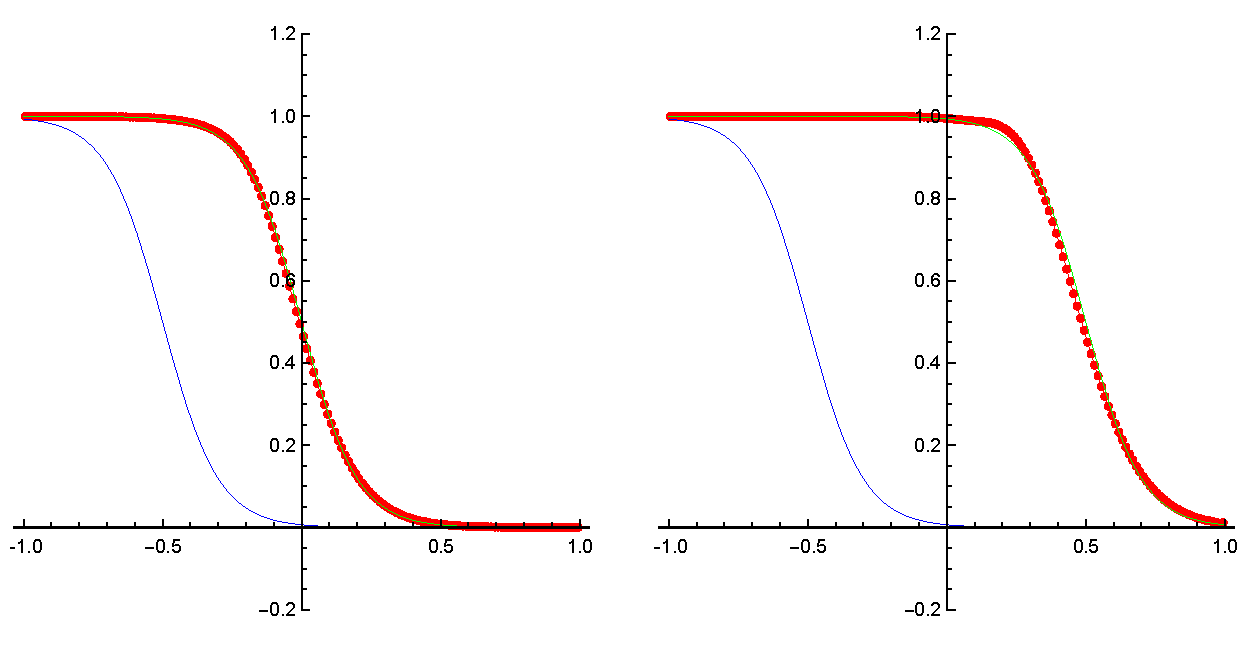
\includegraphics[width=\textwidth]{figures/advection_basic_160c4}
	\caption{Comparing the $\mathrm{IIOE}$ scheme with an exact smooth solution for the linear advection equation \eqref{advection_constant} with constant speed $ v = 1 $ with numerical flux defined by \eqref{iioe_lin_adv_flux} in time $ t=0.5 $(left) and $ t=1 $(right), $ n=160 $, $ \tau=4h $. The initial profile \eqref{lin_adv_smooth_0} is given in blue, the exact solution in green and the numerical solution in red.}
	\label{fig:basic_iioe_advection}
\end{figure}
\textbf{Inviscid Burgers' equation}.  For the nonlinear equation \eqref{inviscid} we chose a smooth rarefaction wave solution with given initial condition
\begin{equation}
	\label{inviscid_smooth_init}
	u^0(x) = \frac{\arctan (10\,x) }{\pi} + 1/2.
\end{equation}
The exact solution can be obtained by the method of characteristics, see, e.g.\ \cite{olv, lev, whitham}. It can be shown, that if the initial profile is non-decreasing everywhere, then the solution does not develop discontinuities for $ t>0 $ \cite{olv, whitham}. The numerical solution was computed on space interval (-2, 2) and time (0, 1). The $ L_1(I, L_1) $ errors and EOC are reported in Table ~\ref{tab:iioe_smooth_nonlinear}. The numerical solution is visually compared to the exact one in Figure ~\ref{fig:iioe_smooth_nonlinear}.
\begin{table}[ht]
	\caption{Report on the $L_1(I, L_1)$ errors of the $\mathrm{IIOE}$ scheme for a smooth rarefaction wave solution of the inviscid Burgers' equation \eqref{inviscid} with numerical flux defined by \eqref{basic_iioe_burgers_flux}, $ \tau = 4h $.}
	\begin{center} \footnotesize
		\begin{tabular}{|c|c|c|c|c|c|}
			\hline
			$ n $ & $ h $ & $ \tau $ & NTS& $\mathrm{L_1(I,L_1)}$ & EOC \\
			\hline
			\lower.3ex\hbox{80} & \lower.3ex\hbox{0.05} & \lower.3ex\hbox{0.2} & \lower.3ex\hbox{5} & \lower.3ex\hbox{2.32 $10^{-2}$} & \\
			\hline
			\lower.3ex\hbox{160} & \lower.3ex\hbox{0.025} & \lower.3ex\hbox{0.1} & \lower.3ex\hbox{10} & \lower.3ex\hbox{6.93 $10^{-3}$} &\lower.3ex\hbox{1.74} \\
			\hline
			\lower.3ex\hbox{320} & \lower.3ex\hbox{0.0125} & \lower.3ex\hbox{0.05} & \lower.3ex\hbox{20} & \lower.3ex\hbox{1.86 $10^{-3}$}  &\lower.3ex\hbox{1.90}\\
			\hline
			\lower.3ex\hbox{640} & \lower.3ex\hbox{0.00625} & \lower.3ex\hbox{0.025} & \lower.3ex\hbox{40} & \lower.3ex\hbox{4.70 $10^{-4}$}  &\lower.3ex\hbox{1.98}\\
			\hline
		\end{tabular}
	\end{center}
	\label{tab:iioe_smooth_nonlinear}
\end{table}
\begin{figure}[H]
	\centering
	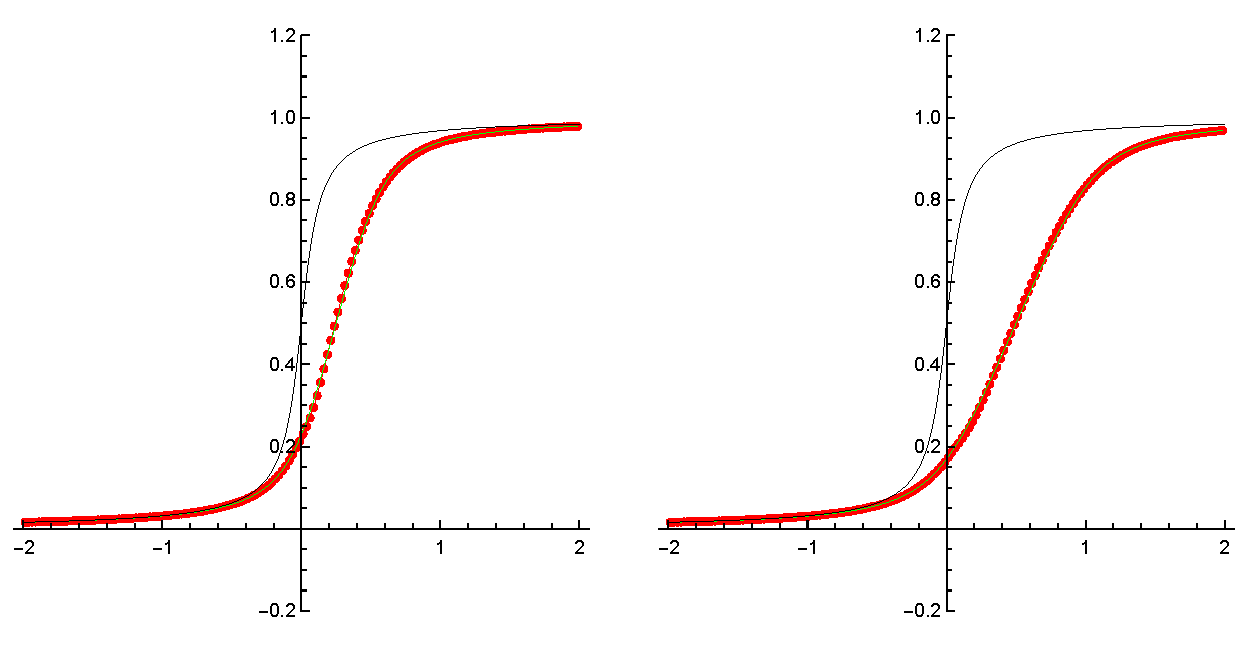
\includegraphics[width=\textwidth]{figures/invBurgSmooth160c4}
	\caption{Comparing the $\mathrm{IIOE}$ scheme with the exact smooth rarefaction wave solution of the inviscid Burgers' equation \eqref{inviscid} with numerical flux defined by \eqref{basic_iioe_burgers_flux} in time $ t=0.5 $(left) and $ t=1 $(right), $ n=160 $, $ \tau=4h $. The initial profile \eqref{inviscid_smooth_init} is given in black, the exact solution in green and the numerical solution in red.}
	\label{fig:iioe_smooth_nonlinear}
\end{figure}
%====================================================================================================================================================
\newpage
\section{Flux Limited IIOE method}
Higher order schemes suffer from numerical dispersion. Nonphysical oscillations can occur near sharp changes of the solution. A remedy to this is to use limiters \cite{lev}.

While calculating the flux at a given interface, previously we took both terms in \eqref{flux_iioe} with equal weight $ 1/2 $. This suggests that we should, as a possible improvement, calculate a weighted average instead:
\begin{equation}
	\label{limited_flux}
	F_{i - 1/2}^{\theta} = 
\begin{cases}
	(1-\theta_{i-1/2})f^n_{i-1} + \theta_{i-1/2} f^{n-1}_{i} &  \text{if } f'(u)\big|_{\substack{x_{i-1/2}}} > 0\\
	\\
	\theta_{i-1/2} f^{n-1}_{i-1} + (1-\theta_{i-1/2}) f^{n}_{i} &  \text{if } f'(u)\big|_{\substack{x_{i-1/2}}} < 0
\end{cases}
\end{equation}
for some weighting coefficient $ \theta_{i-1/2} $. One should notice that for $ \theta_{i-1/2} = \frac{1}{2} $ we get the basic IIOE scheme and for $ \theta_{i-1/2} = 0 $ we get the implicit upwind scheme.\\
It is important that we assign a weighting coefficient to a given interface, so the method stays conservative. This is not true for the limiter used in previous works \cite{iioe2012, iioe2}.

\textbf{Remark}. The weighted averaging of implicit and explicit terms in \eqref{limited_flux} can be interpreted as a flux-limiter method \cite{lev}, where we combine a high-order scheme with a low-order one. The goal is to use the higher-order scheme as much as possible without generating nonphysical oscillations. The flux is calculated as follows:
\begin{equation}
	\label{flux_limiter}
	F^{\Phi}_{i-1/2} = F^L_{i-1/2} + \Phi_{i-1/2} (F^H_{i-1/2} - F^L_{i-1/2}),
\end{equation}
where $ F^L_{i-1/2} $ is a flux of a low-order scheme, which does not make new minima or maxima, neither accentuates already existing ones, $ F^H_{i-1/2} $ is a high-order flux, which is more accurate but nonphysical oscillations might occur in the numerical solution, $ \Phi_{i-1/2} $ is a flux limiter $ 0 \leq \Phi_{i-1/2} \leq 1 $. Notice that for $ \Phi_{i-1/2} = 0 $ the flux consists only of the low-order flux, for $ \Phi_{i-1/2} = 1 $ we have the higher-order flux.
The weighted averaging in \eqref{limited_flux} described previously is equivalent to flux-limiter method, if the flux of the  higher-order scheme is the basic IIOE \eqref{flux_iioe} and the low-order flux comes from the implicit upwind scheme. Then the limited flux \eqref{flux_limiter} for $ f'(u) > 0 $ can be written as
\begin{equation}
	\begin{split}
	F^{\Phi}_{i-1/2} &= f(u^n_{i-1}) + \Phi_{i-1/2} \left(\frac{1}{2} f(u^n_{i-1}) + \frac{1}{2} f(u^{n-1}_{i}) - f(u^n_{i-1})\right)\\
				   	 &= \left(1 - \frac{\Phi_{i-1/2}}{2}\right) f(u^n_{i-1}) + \frac{\Phi_{i-1/2}}{2} f(u^{n-1}_{i}).
	\end{split}
\end{equation}
We can see that the two approaches are equivalent by choosing $ \theta_{i-1/2} = \frac{\Phi_{i-1/2}}{2} $. This implies that we should expect that our weighting coefficient is bounded $ 0 \leq \theta_{i-1/2} \leq 1/2 $. We calculate $ F^{\Phi}_{i+1/2} $ analogously.

An interesting question is how to calculate the weighting coefficient. We can use a similar approach as in \cite{borisbook, zalesak, iioe2012, iioe2}, which means that we calculate the weighting coefficients in a way to ensure that the numerical solution does not accentuates existing minima and maxima.
\subsection{Advection with constant speed}
Here we present a possible way for the limiting process in case of linear advection \eqref{advection_constant}, considering the characteristic speed $ v > 0 $ is positive everywhere. In this case the scheme reads
\begin{equation}
	\label{advection_limit}
	u_i^{n} = u_i^{n - 1} - v \frac{\tau}{h} \left[\left((1 - \theta_{i+1/2})u^n_{i} + \theta_{i+1/2}u^{n-1}_{i+1}\right) - \left((1 - \theta_{i-1/2})u^n_{i-1} + \theta_{i-1/2}u^{n-1}_{i}\right)\right].
\end{equation}
In this case the only unknowns in the equation are the weighting coefficients and the value $ u_i^n $. We calculate the weighting coefficients to ensure that the value in the new time step will not be greater as an appropriately defined maximum value $ u_{i,max}^n $ neither smaller then a minimum value $ u_{i,min}^n $, i.e.\
\[
u_{i,min}^n \leq u^n_i \leq u_{i,max}^n.
\]
A simple choice for $ u_{i,min}^n,\, u_{i,max}^n $ is for example
\[
u_{i,min}^n = \min(u_{i-\left \lfloor{c}\right \rfloor}^{n-1},\, u_{i-\left \lfloor{c}\right \rfloor -1}^{n-1}),\quad
u_{i,max}^n = \max(u_{i-\left \lfloor{c}\right \rfloor}^{n-1},\, u_{i-\left \lfloor{c}\right \rfloor-1}^{n-1})
\]
where $ c $ is the Courant number $ c = v \tau/h $. We apply the floor function $ \left \lfloor{c}\right \rfloor $, which returns the largest integer less then or equal to $ c $. A similar approach was used in \cite{iioe2012, iioe2}. We start the calculation at the left end of the interval, which is the inflow boundary, where we know the value $ u_0^n $ from the given Dirichlet boundary condition. We set $ \theta_{1/2} = 1/2,\, \theta_{3/2} = 1/2$, which means that we calculate $ u_1^n $ with the basic IIOE scheme. If $ u_1^n < u_{i,min}^n $ we adjust $ \theta_{3/2} $ in order to get $ u_1^n \geq u_{i,min}^n $. The case if $ u_1^n > u_{i,max}^n $ is treated analogously. \\
Below we describe the steps of our flux limiting approach, the $ \mathrm{FLIIOE} $ method. In general, for the $ i $-th cell we do the following:
\begin{enumerate}
	\item $ u_{i-1}^n $ and $\theta_{i-1/2}$ are known.
	\item Set $ \theta_{i+1/2}=1/2 $.
	\item Calculate $ u_i^n $ from \eqref{advection_limit}
	\begin{equation}
		\label{u_i^n_linear}
		u_i^n = \frac{u_i^{n - 1} - 
		c
		\left[\theta_{i+1/2}u^{n-1}_{i+1} -
		(1 - \theta_{i-1/2})u^n_{i-1} - \theta_{i-1/2}u^{n-1}_{i}
		\right]}{1+ c(1 - \theta_{i+1/2})}.
	\end{equation}
	\item If $ u_i^n < u_{i,min}^n $ it is desired that
	\[u_{i,min}^n \leq \frac{u_i^{n - 1} - 
		c
		\left[\theta_{i+1/2}u^{n-1}_{i+1} -
		(1 - \theta_{i-1/2})u^n_{i-1} - \theta_{i-1/2}u^{n-1}_{i}
		\right]}{1+ c(1 - \theta_{i+1/2})},
	\]
from which we get
\[
\theta_{i+1/2} \leq \frac{u_i^{n-1} + c\left(\theta_{i-1/2}u^n_{i-1} + \theta_{i-1/2}u^{n-1}_{i}\right) - u_{i,min}^n(1+c)}{c(u_{i+1}^{n-1} - u_{i,min}^n)}.
\]
Thus we redefine
\begin{equation}
	\hspace{-20mm}\theta_{i+1/2} = \min \left(\max\left(\frac{u_i^{n-1} + c\left(\theta_{i-1/2}u^n_{i-1} + \theta_{i-1/2}u^{n-1}_{i}\right) - u_{i,min}^n(1+c)}{c(u_{i+1}^{n-1} - u_{i,min}^n)},0\right),1/2\right).
\end{equation}
\item If $ u_i^n > u_{i,max}^n $ it is desired that
\[u_{i,max}^n \geq \frac{u_i^{n - 1} - 
	c
	\left[\theta_{i+1/2}u^{n-1}_{i+1} -
	(1 - \theta_{i-1/2})u^n_{i-1} - \theta_{i-1/2}u^{n-1}_{i}
	\right]}{1+ c(1 - \theta_{i+1/2})},
\]
from which we get
\[
\theta_{i+1/2} \geq \frac{u_i^{n-1} + c\left(\theta_{i-1/2}u^n_{i-1} + \theta_{i-1/2}u^{n-1}_{i}\right) - u_{i,max}^n(1+c)}{c(u_{i+1}^{n-1} - u_{i,max}^n)}.
\]
Thus we redefine
\begin{equation}
	\hspace{-20mm}\theta_{i+1/2} = \min \left(\max\left(\frac{u_i^{n-1} + c\left(\theta_{i-1/2}u^n_{i-1} + \theta_{i-1/2}u^{n-1}_{i}\right) - u_{i,max}^n(1+c)}{c(u_{i+1}^{n-1} - u_{i,max}^n)},0\right),1/2\right).
\end{equation}
\item We calculate $ u_i^n $ by \eqref{u_i^n_linear} as in step 3 with a possibly modified $ \theta_{i+1/2} $.
\end{enumerate}
\begin{comment}
The procedure discussed above sets the solution $ u_i^n $ to $ u_{i,min}^n $, if it would be smaller, or $ u_{i,max}^n $, if it would be greater. The second approach we propose is based on the idea that if the solution is outside the interval $ (u_{i, min}^n, u_{i, max}^n) $, we adjust $ \theta_{i+1/2} $ according to the Courant number $ c $, which tells us where the information comes from. If $ c $ is not an integer, we expect the solution to be inside $ (u_{i-\left \lfloor{c}\right \rfloor}^{n-1},\, u_{i-\left \lfloor{c}\right \rfloor-1}^{n-1}) $. For that reason, we modify the previous procedure. In our second flux limiting approach, denoted by $ \mathrm{FL^2 IIOE} $, we replace steps 4 and 5 in the previous algorithm with
\begin{itemize}
	\item we define
	\[
	u_{i,c}^n = (c - \left \lfloor{c}\right \rfloor)u_{i-\left \lfloor{c}\right \rfloor - 1}^{n-1} + (1 - (c - \left \lfloor{c}\right \rfloor))u_{i-\left \lfloor{c}\right \rfloor}^{n-1},
	\]
	which is a simple linear interpolation between the values.
	\item if $ u_{i,c}^n - u_{i+1}^{n-1} \neq 0 $ and ($ u_i^n > u_{i,max}^n $ or $ u_i^n < u_{i,min}^n $) we define
	\begin{equation}
		\hspace{-20mm}\theta_{i+1/2} = \min \left(\max\left(\frac{u_i^{n-1} + c\left(\theta_{i-1/2}u^n_{i-1} + \theta_{i-1/2}u^{n-1}_{i}\right) - u_{i,c}^n(1+c)}{c(u_{i+1}^{n-1} - u_{i,c}^n)},0\right),1/2\right).
	\end{equation}
\end{itemize}
\end{comment}
We performed numerical experiments in section 2.5.3. 
%==============================================================================================================================================================================================================================================================
\subsection{Inviscid Burgers' equation}
We describe a possible way to limit the scheme also in the case of a nonlinear equation. Again, for simplicity we assume that the characteristic speed $ f'(u) = u \geq 0 $ is non-negative everywhere The scheme then reads
\begin{multline}
	\label{burgers_limit}
	u_i^{n} = u_i^{n - 1} - \frac{\tau}{h}\biggl[\left((1 - \theta_{i+1/2})\frac{(u^n_{i})^2}{2} + \theta_{i+1/2}\frac{(u^{n-1}_{i+1})^2}{2} \right)\\	- \left((1 - \theta_{i-1/2})\frac{(u^n_{i-1})^2}{2} + \theta_{i-1/2}\frac{(u^{n-1}_{i})^2}{2}\right)\biggr]
\end{multline}
We use similar ideas as in the case of linear transport. We want to ensure that our numerical solution does not violate the min-max principle. Since the speed is not constant, we calculate $ u_{i,min}^n $ and $ u_{i,max}^n $ differently. First we calculate the Courant number using the maximum value of the characteristic speed at the previous time step, which is $ \max_i(u_i^{n-1}) $ in the case of the inviscid Burgers' equation. We calculate the maximal Courant number 
\begin{equation}
	\label{courant_burgers}
	 c=\max_i(u_i^{n-1}) \tau /h.
\end{equation}
Then the limiting values are calculated as
\[
u_{i,min}^n = \min_{i- \left \lfloor{c}\right \rfloor - 1}^{i}(u_i^{n-1}),\quad
u_{i,max}^n = \max_{i- \left \lfloor{c}\right \rfloor - 1}^{i}(u_i^{n-1}).
\]
The procedure is then analogous to the linear case, except we use \eqref{burgers_limit}. Below we describe the steps of the flux limiting $\mathrm{FLIIOE} $ method for the inviscid Burgers' equation. In general, for the $ i $-th cell we do the following:
\begin{enumerate}
	\item $ u_{i-1}^n $ and $ \theta_{i-1/2} $ are known.
	\item We set $ \theta_{i+1/2} = 1/2 $.
	\item Calculate $ u_i^n $ from \eqref{burgers_limit}
	\begin{equation}
		\label{u_i^n_burgers}
		u_i^n = \frac{-1 \pm \sqrt{1+\frac{\tau}{h}(1-\theta_{i+1/2})(\frac{\tau}{h}F^{\theta}_{i-1/2} +2 u_i^{n-1}-\frac{\tau}{h}\theta_{i+1/2} (u_{i+1}^{n-1})^2)}}{\frac{\tau}{h}(1-\theta_{i+1/2})},
	\end{equation}
	where 
	 \[F^{\theta}_{i-1/2} = (1 - \theta_{i-1/2})\frac{(u^n_{i-1})^2}{2} + \theta_{i-1/2}\frac{(u^{n-1}_{i})^2}{2}.\]
	\begin{itemize}
		\item We have to decide, which solution to choose. Since the numerical experiments we performed all have positive initial values, we chose the positive one from the two.
		\item If the expression under the square root is negative, we fail to calculate a real solution. In this case we set $ \theta_{i+1/2} = 0 $, i.e.\ at $ x_{i-1/2} $ we use the implicit upwind flux.
	\end{itemize}
	\item If $ u_i^n < u_{i,min}^n $ it is desired that
	\[
	u_{i,min}^n \leq \frac{-1 + \sqrt{1+\frac{\tau}{h}(1-\theta_{i+1/2})(\frac{\tau}{h}F^{\theta}_{i-1/2} +2 u_i^{n-1}-\frac{\tau}{h}\theta_{i+1/2} (u_{i+1}^{n-1})^2)}}{\frac{\tau}{h}(1-\theta_{i+1/2})},
	\]
	from which we get
	\begin{equation}
			\theta_{i+1/2} \leq \frac{u_i^{n-1} - u_{i,min}^n + \frac{\tau}{h}(F^{\theta}_{i-1/2} - (u_{i,min}^n)^2/2)}{\frac{\tau}{2h}((u_{i,min}^n)^2 - (u_{i+1}^{n-1})^2)}.
	\end{equation}
	Thus we redefine
	\begin{equation}
		\theta_{i+1/2} = \min \left(\max\left(\frac{u_i^{n-1} - u_{i,min}^n + \frac{\tau}{h}(F^{\theta}_{i-1/2} - (u_{i,min}^n)^2/2)}{\frac{\tau}{2h}((u_{i,min}^n)^2 - (u_{i+1}^{n-1})^2)},0\right),1/2\right).
	\end{equation}
	\item If $ u_i^n > u_{i,max}^n $ we want
	\[
	u_{i,max}^n \geq \frac{-1 + \sqrt{1+\frac{\tau}{h}(1-\theta_{i+1/2})(\frac{\tau}{h}F^{\theta}_{i-1/2} +2 u_i^{n-1}-\frac{\tau}{h}\theta_{i+1/2} (u_{i+1}^{n-1})^2)}}{\frac{\tau}{h}(1-\theta_{i+1/2})},
	\]
	from which we get
	\begin{equation}
			\theta_{i+1/2} \geq \frac{u_i^{n-1} - u_{i,max}^n + \frac{\tau}{h}(F^{\theta}_{i-1/2} - (u_{i,max}^n)^2/2)}{\frac{\tau}{2h}((u_{i,max}^n)^2 - (u_{i+1}^{n-1})^2)}.
	\end{equation}
	Thus we redefine
	\begin{equation}
		\theta_{i+1/2} = \min \left(\max\left(\frac{u_i^{n-1} - u_{i,max}^n + \frac{\tau}{h}(F^{\theta}_{i-1/2} - (u_{i,max}^n)^2/2)}{\frac{\tau}{2h}((u_{i,max}^n)^2 - (u_{i+1}^{n-1})^2)},0\right),1/2\right).
	\end{equation}
	\item We calculate $ u_i^n $ by \eqref{u_i^n_burgers} with a possibly modified $ \theta_{i+1/2} $.
\end{enumerate}
\begin{comment}
As in the case of the linear problem, the procedure discussed above sets the solution $ u_i^n $ to $ u_{i,min}^n $, if it would be smaller, or $ u_{i,max}^n $, if it would be greater. Since it is not necessary for the solution to be equal to $ u_{i,min}^n $ or $ u_{i,max}^n $, we expect that it can be between them. Thus we modify the first procedure, so that we replace steps 4, 5 of $ \mathrm{FL^1 IIOE} $ in our second flux limiting approach $ \mathrm{FL^2 IIOE} $ with
\begin{itemize}
	\item We define 
	\[
	u_{i,c}^n = u_{i- \left \lfloor{c + 0.5}\right \rfloor},
	\]
	where $ \left \lfloor{c + 0.5}\right \rfloor $ rounds $ c $, calculated as \eqref{courant_burgers}, to the nearest integer.
	\item if $ u_{i,c}^n - u_{i+1}^{n-1} \neq 0 $ and ($ u_i^n > u_{i,max}^n $ or $ u_i^n < u_{i,min}^n $) we define
	\begin{equation}
		\theta_{i+1/2} = \min \left(\max\left(\frac{u_i^{n-1} - u_{i,c}^n + \frac{\tau}{h}(F^{\theta}_{i-1/2} - (u_{i,c}^n)^2/2)}{\frac{\tau}{2h}((u_{i,c}^n)^2 - (u_{i+1}^{n-1})^2)},0\right),1/2\right),
	\end{equation}
	where we replaced $ u_{i, min}^n $ or $ u_{i, max}^n $ with $ u_{i, c}^n $.
\end{itemize}
\end{comment}
We performed numerical experiments in section 2.5.4.
%=================================================================================================================================================================================
\subsection{Numerical experiments - Advection with constant speed}
In this section we present numerical experiments performed by the flux limited $ \mathrm{FLIIOE} $ scheme in case of advection with constant speed. In this linear case \eqref{advection_limit} is compared with the stabilized schemes $ \mathrm{S^1IIOE} $ (without quadratic reconstruction) and $ \mathrm{S^2IIOE} $ (with quadratic reconstruction) described in \cite{iioe2012,iioe2}. For this purpose we use the same examples that can be found in these works: a \textbf{smooth profile} with initial condition 
\begin{equation}
	\label{advection_smooth}
u^0(x) = \mathrm{max}(0, \cos^5(\pi(x+0.5))),
\end{equation}
and a \textbf{piecewise constant profile} with initial condition
\begin{equation}
	\label{advection_piece}
	u^0(x) =
	\begin{cases}
		1, &x\in[-0.75, -0.25],\nonumber\\
		0, &\textrm{otherwise}.\nonumber
	\end{cases}
\end{equation}
In both cases we solve \eqref{advection_constant} numerically with $ v = 1 $ on space interval $ (-1,1) $ and time interval $ (0,1) $. The exact solution is calculated as $ u(t, x) = u^0(x - t) $. At the inflow boundary exact Dirichlet boundary condition is given.\\
The values for $ \mathrm{S^2IIOE} $ (with quadratic reconstruction) are taken from previous works \cite{iioe1,iioe2}. 
For the smooth profile \eqref{advection_smooth} we can observe that the flux limited scheme \eqref{advection_limit} performs better than the $ \mathrm{S^1IIOE} $ and it is comparable with the $ \mathrm{S^2IIOE} $ in all cases. The results are documented in Table ~\ref{tab:siioe_hump}. In Figure  ~\ref{fig:compare_S1FL_hump} we compare $ \mathrm{S^1IIOE} $ with the flux limited scheme \eqref{advection_limit} visually.\\
In the case of a discontinuous profile \eqref{advection_piece} the flux limited scheme \eqref{advection_limit} performs better than both stabilized schemes, c.f.\ Table  ~\ref{tab:siioe_disc}. A visual comparison with $ \mathrm{S^1 IIOE} $ can be seen in Figure ~\ref{fig:compare_S1FL_disc}.
\begin{table}[ht]
	\caption{Report on the $L_1(I, L_1)$ errors of the $\mathrm{S^1 IIOE}$ scheme without quadratic reconstruction, $\mathrm{S^2 IIOE}$ scheme with quadratic reconstruction, the flux limited $\mathrm{FLIIOE}$ scheme \eqref{advection_limit} for a smooth initial profile \eqref{advection_smooth}, $ \tau = h $.}
	\begin{center} \footnotesize
\begin{tabular}{|c|c|c|c|c|c|c|}
\hline
& $ \mathrm{S^1 IIOE} $ &$ \mathrm{S^1 IIOE} $ & $ \mathrm{S^2 IIOE} $ &$ \mathrm{S^2 IIOE} $ & $ \mathrm{FLIIOE} $ & $ \mathrm{FLIIOE} $ \\
$ n $ & $\mathrm{L_1(I, L_1)}$ & EOC & $\mathrm{L_1(I, L_1)}$ & EOC & $\mathrm{L_1(I, L_1)}$ & EOC \\
\hline
\lower.3ex\hbox{40} &  \lower.3ex\hbox{9.82 $10^{-2}$} & & \lower.3ex\hbox{9.19 $10^{-2}$} & & \lower.3ex\hbox{7.27 $10^{-2}$} &\\
\hline
\lower.3ex\hbox{80} &  \lower.3ex\hbox{3.38 $10^{-2}$} &\lower.3ex\hbox{1.54} & \lower.3ex\hbox{2.80 $10^{-2}$} &\lower.3ex\hbox{1.71}&\lower.3ex\hbox{2.63 $10^{-2}$}& \lower.3ex\hbox{1.47} \\
\hline
\lower.3ex\hbox{160} &  \lower.3ex\hbox{1.01 $10^{-2}$} &\lower.3ex\hbox{1.74}& \lower.3ex\hbox{7.69 $10^{-3}$} &\lower.3ex\hbox{1.86} &\lower.3ex\hbox{7.55 $10^{-3}$}& \lower.3ex\hbox{1.80} \\
\hline
\lower.3ex\hbox{320} &  \lower.3ex\hbox{2.73 $10^{-3}$} &\lower.3ex\hbox{1.89}& \lower.3ex\hbox{1.97 $10^{-3}$} &\lower.3ex\hbox{1.96} &\lower.3ex\hbox{1.96 $10^{-3}$}& \lower.3ex\hbox{1.95}\\
\hline
\lower.3ex\hbox{640} &  \lower.3ex\hbox{7.11 $10^{-4}$} &\lower.3ex\hbox{1.94}& \lower.3ex\hbox{4.97 $10^{-4}$} &\lower.3ex\hbox{1.99} &\lower.3ex\hbox{5.22 $10^{-4}$}& \lower.3ex\hbox{1.91}\\
\hline
\lower.3ex\hbox{1280} &  \lower.3ex\hbox{1.83 $10^{-4}$} &\lower.3ex\hbox{1.96}& \lower.3ex\hbox{1.24 $10^{-4}$} &\lower.3ex\hbox{2.00} &\lower.3ex\hbox{1.41 $10^{-4}$}& \lower.3ex\hbox{1.89}\\
\hline
\end{tabular}
\end{center}
\label{tab:siioe_hump}
\end{table}

\begin{figure}[H]
	\centering
	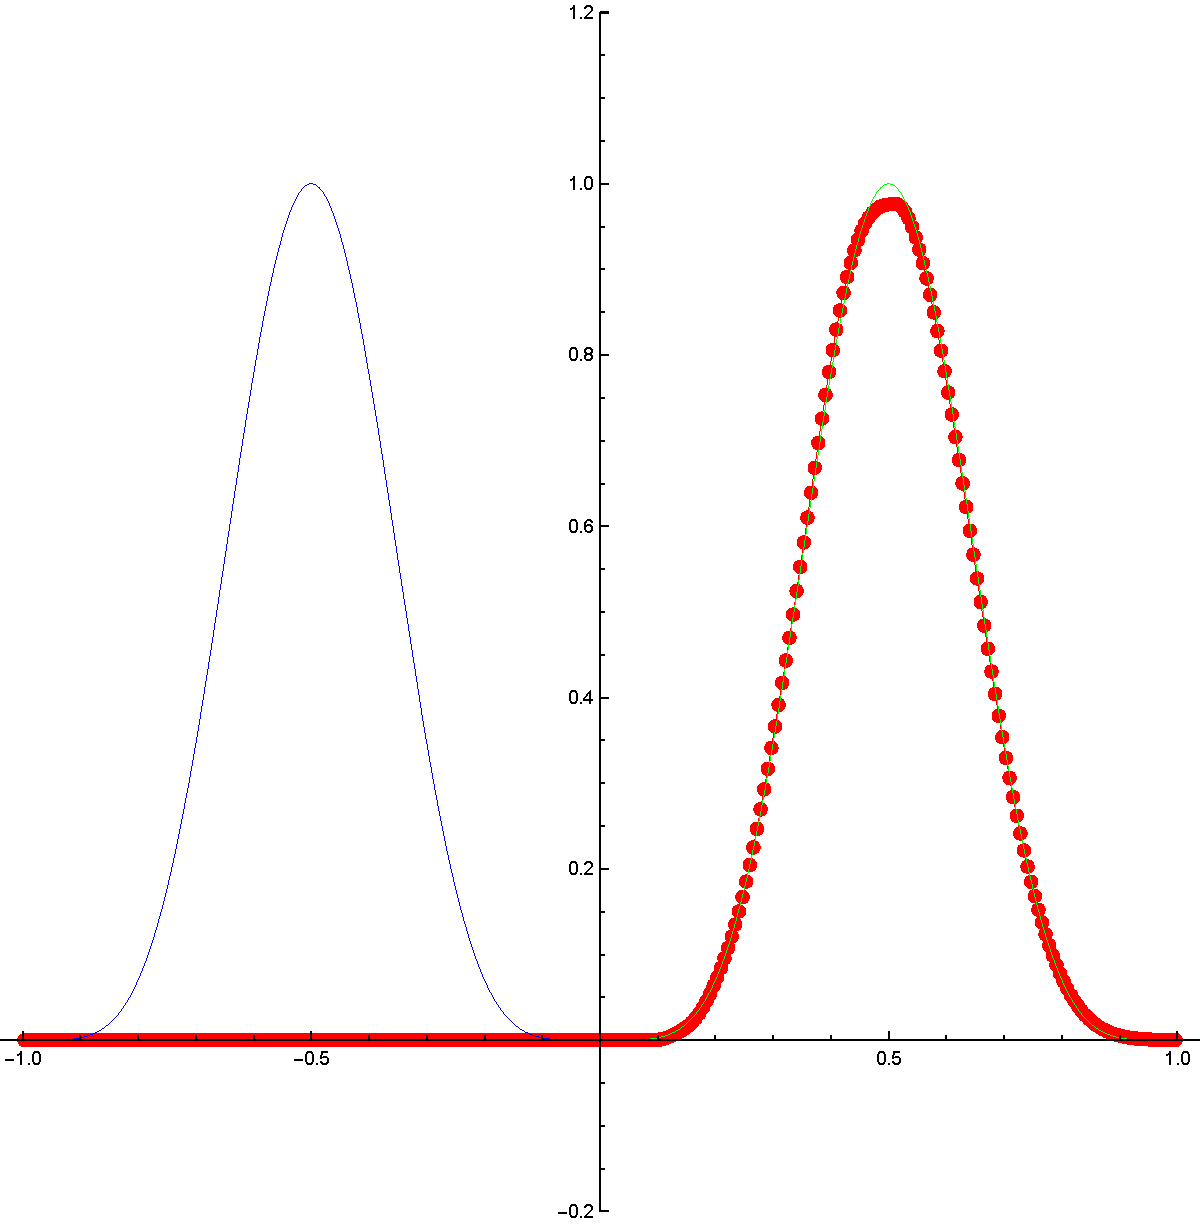
\includegraphics[width=.49\textwidth]{figures/smooth(S1IIOE)_320_h}
	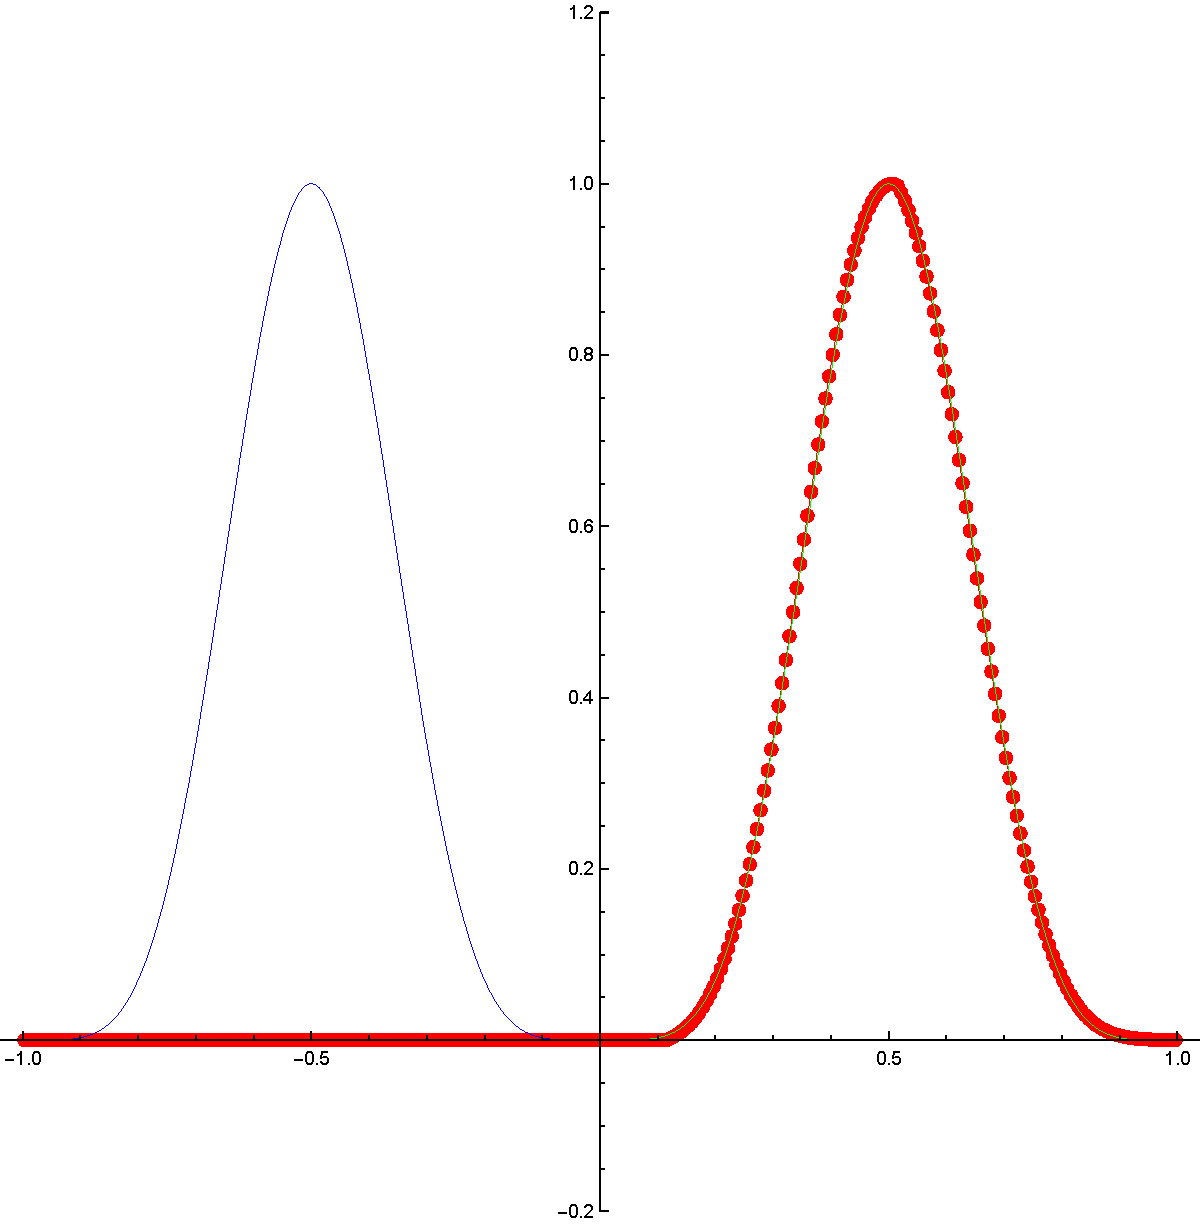
\includegraphics[width=.49\textwidth]{figures/hump_320_h}
	\caption{Comparing the $\mathrm{S^1 IIOE}$ scheme without quadratic reconstruction (left) and the flux limited $\mathrm{FLIIOE}$ scheme \eqref{advection_limit} (right) with the exact solution of \eqref{advection_constant} for a smooth initial profile \eqref{advection_smooth} in time $ t=1 $, $ n=320 $, $ \tau=h $.}
	\label{fig:compare_S1FL_hump}
\end{figure}

\begin{table}[ht]
	\caption{Report on the $L_1(I, L_1)$ errors of the $\mathrm{S^1 IIOE}$ scheme without quadratic reconstruction, $\mathrm{S^2 IIOE}$ scheme with quadratic reconstruction and the flux limited $\mathrm{FLIIOE}$ scheme \eqref{advection_limit} for a piecewise constant initial profile \eqref{advection_piece}, $ \tau = h $.}
	\begin{center} \footnotesize
		\begin{tabular}{|c|c|c|c|c|c|c|}
			\hline
			& $ \mathrm{S^1 IIOE} $ &$ \mathrm{S^1 IIOE} $ & $ \mathrm{S^2 IIOE} $ &$ \mathrm{S^2 IIOE} $ & $ \mathrm{FLIIOE} $ & $ \mathrm{FLIIOE} $ \\
			$ n $ & $\mathrm{L_1 error}$ & EOC & $\mathrm{L_1 error}$ & EOC & $\mathrm{L_1 error}$ & EOC \\
			\hline
			\lower.3ex\hbox{40} &  \lower.3ex\hbox{2.03 $10^{-1}$} & & \lower.3ex\hbox{2.02 $10^{-1}$} & & \lower.3ex\hbox{1.49 $10^{-1}$}&\\
			\hline
			\lower.3ex\hbox{80} &  \lower.3ex\hbox{1.31 $10^{-1}$} &\lower.3ex\hbox{0.63}& \lower.3ex\hbox{1.30 $10^{-1}$} &\lower.3ex\hbox{0.63}& \lower.3ex\hbox{9.40 $10^{-2}$} & \lower.3ex\hbox{0.66}\\
			\hline
			\lower.3ex\hbox{160} &  \lower.3ex\hbox{8.38 $10^{-2}$} &\lower.3ex\hbox{0.64}& \lower.3ex\hbox{8.38 $10^{-2}$} &\lower.3ex\hbox{0.64}& \lower.3ex\hbox{5.91 $10^{-2}$} &\lower.3ex\hbox{0.67}\\
			\hline
			\lower.3ex\hbox{320} &  \lower.3ex\hbox{5.35 $10^{-2}$} &\lower.3ex\hbox{0.65}&  \lower.3ex\hbox{5.34 $10^{-2}$} &\lower.3ex\hbox{0.65}& \lower.3ex\hbox{3.72 $10^{-2}$} &\lower.3ex\hbox{0.67} \\
			\hline
			\lower.3ex\hbox{640} &  \lower.3ex\hbox{3.41 $10^{-2}$} &\lower.3ex\hbox{0.65}&  \lower.3ex\hbox{3.41 $10^{-2}$} &\lower.3ex\hbox{0.65}& \lower.3ex\hbox{2.35 $10^{-2}$} &\lower.3ex\hbox{0.66}\\
			\hline
			\lower.3ex\hbox{1280} &  \lower.3ex\hbox{2.16 $10^{-2}$} &\lower.3ex\hbox{0.66}& \lower.3ex\hbox{2.16 $10^{-2}$} &\lower.3ex\hbox{0.66}& \lower.3ex\hbox{1.48 $10^{-2}$} &\lower.3ex\hbox{0.67}\\
			\hline
		\end{tabular}
	\end{center}
	\label{tab:siioe_disc}
\end{table}

\begin{figure}[h!]
	\centering
	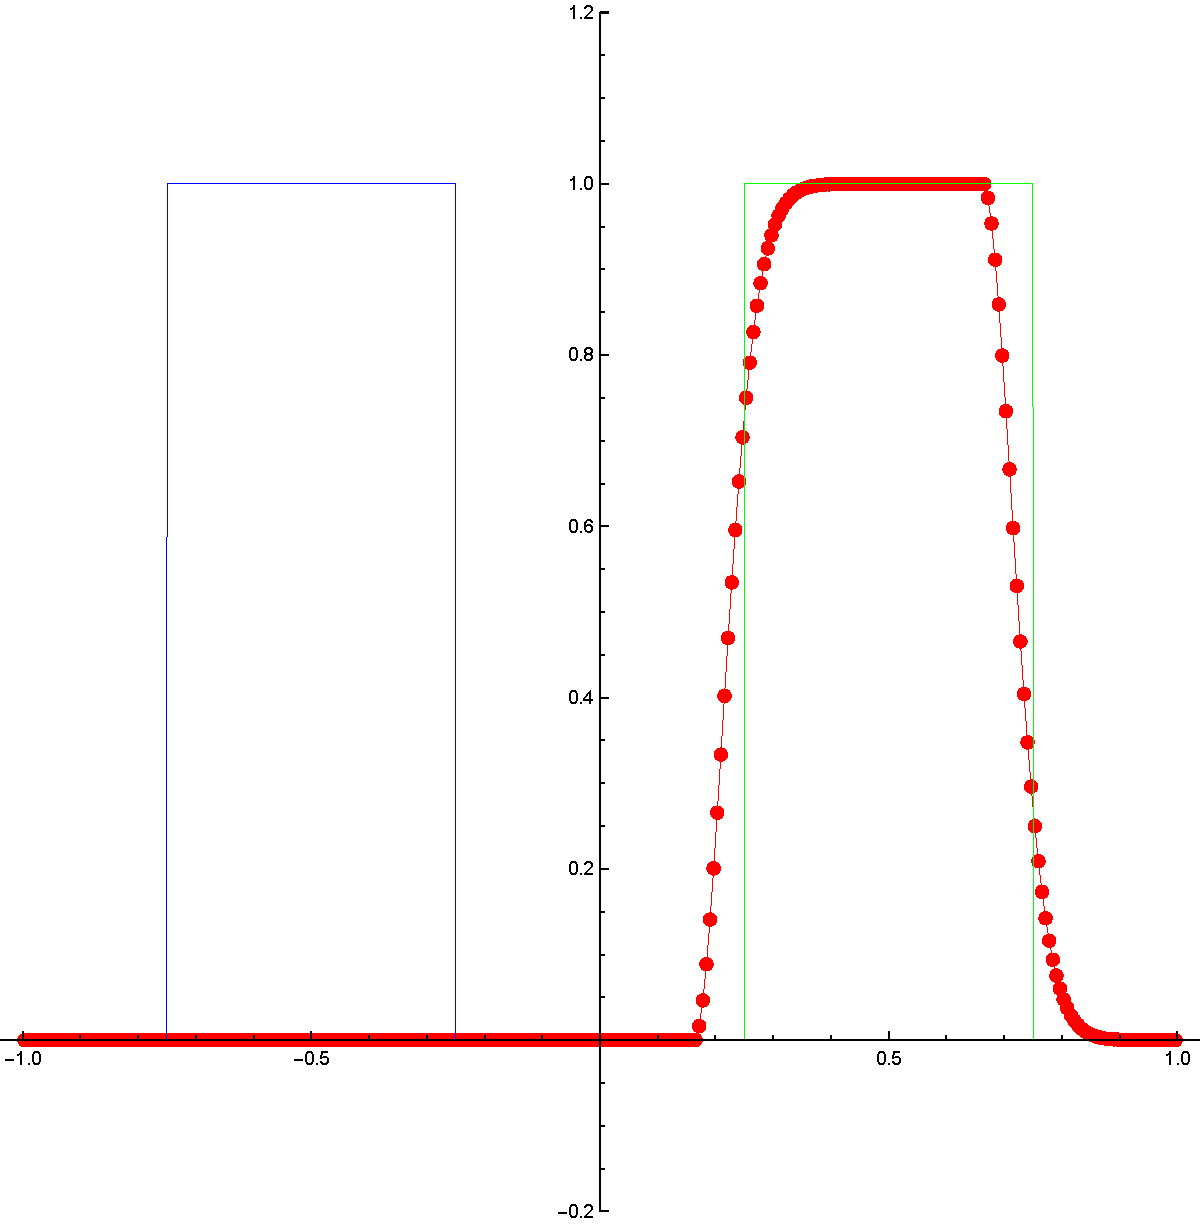
\includegraphics[width=.49\textwidth]{figures/piece(S1IIOE)_320_h}
	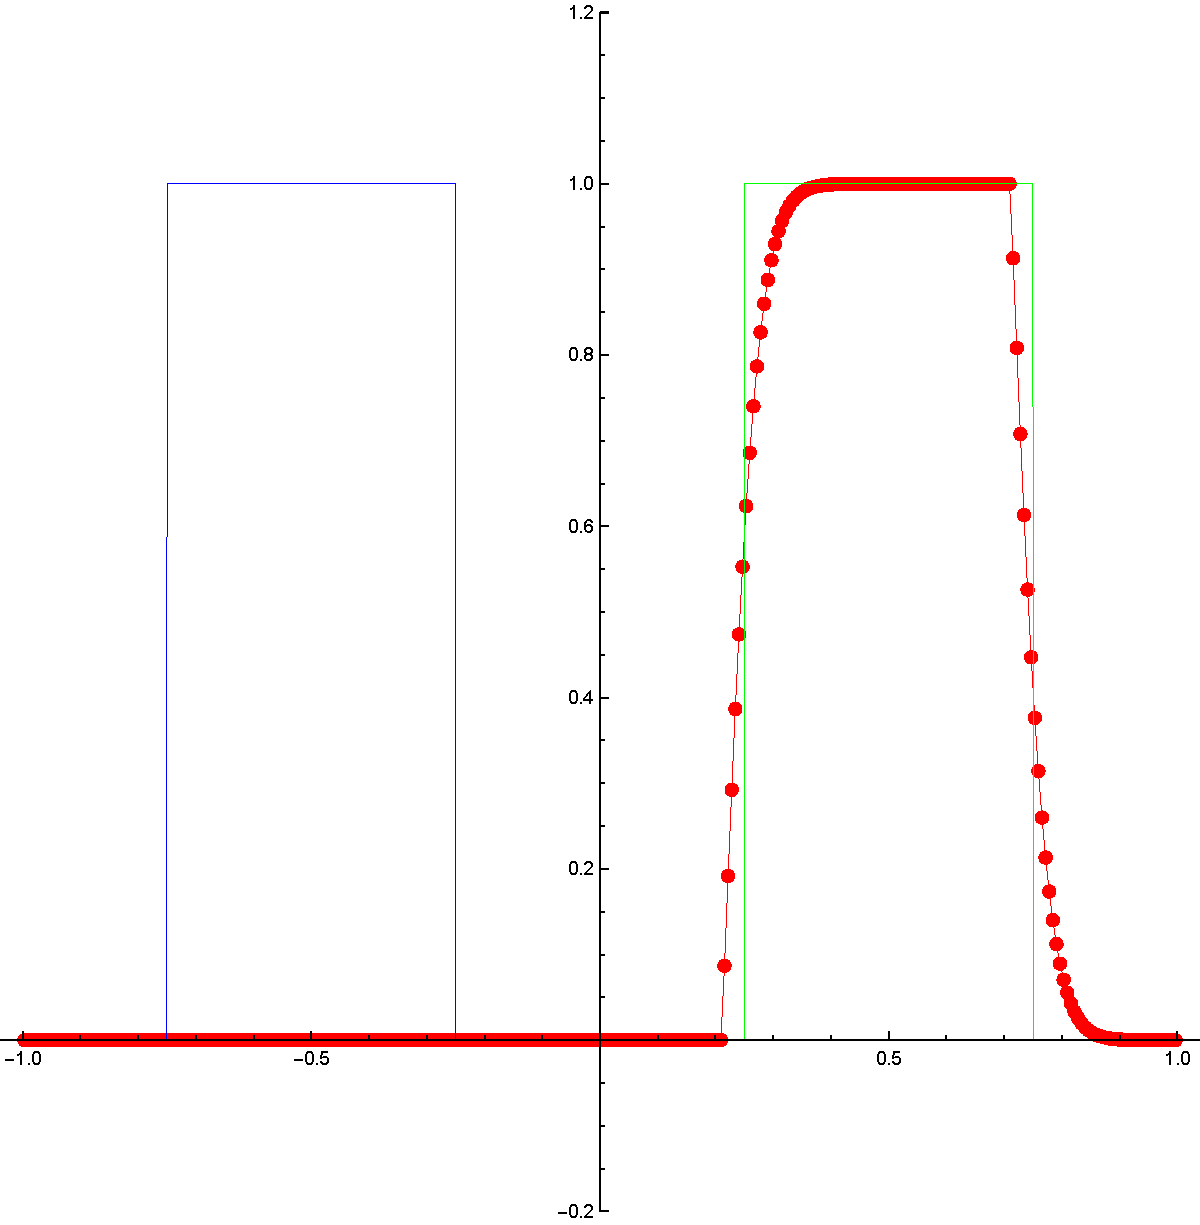
\includegraphics[width=.49\textwidth]{figures/piece_320_h}
	\caption{Comparing the $\mathrm{S^1 IIOE}$ scheme without quadratic reconstruction (left) and the $\mathrm{FLIIOE}$ scheme \eqref{advection_limit} (right) with the exact solution of \eqref{advection_constant} with a piecewise constant initial profile \eqref{advection_piece} in time $ t=1 $, $ n=320 $, $ \tau=h $.}
	\label{fig:compare_S1FL_disc}
\end{figure}
\newpage
\subsection{Numerical experiments - Inviscid Burgers' equation} 

We performed numerical experiments also for the nonlinear transport equation \eqref{inviscid}. For this purpose the following examples where chosen: shock wave, rarefaction wave and triangular wave. As in the linear case, at the inflow boundary exact Dirichlet boundary condition is given.

\textbf{Shock wave}. In this case the scheme \eqref{burgers_limit} is solved on the space interval $ (-0.5,\, 0.5) $ and time interval $ (0, 0.5) $ with a step function initial condition
\begin{equation}
	\label{inviscid_shock_sol}
	u^0(x) =
	\begin{cases}
		1, &x\leq 0,\nonumber\\
		0, &x>0.\nonumber
	\end{cases}
\end{equation}
A physically relevant weak solution \cite{olv, lev, whitham} is a traveling shock wave 
\[
u(t,x)=u^0(x - s\,t),
\]
where $ s = 1/2 $ is the speed of the shock propagation. The $ \mathrm{L_1(I,L_1)} $ errors and EOC of the computation are documented in Table ~\ref{tab:fliioe_invBurg_shock}. A visual comparison of the numerical solution with the exact one can be seen in Figure ~\ref{fig:fliioe_burg_shock}.
\begin{table}[ht]
	\caption{Report on the $L_1(I,L_1)$ errors of the flux limited $\mathrm{FLIIOE}$ scheme \eqref{burgers_limit} for a shock wave solution \eqref{inviscid_shock_sol} of the inviscid Burgers' equation \eqref{inviscid}. We used time steps $ \tau = 4h $ in the first 4 rows and $ \tau = 32h $ in the next 4 rows.}
	\begin{center} \footnotesize
		\begin{tabular}{|c|c|c|c|c|c|}
			\hline
			$ n $ & $ h $ & $ \tau $ & NTS& $\mathrm{L_1(I,L_1)}$ & EOC \\
			%c=4
			\hline
			\lower.3ex\hbox{80} & \lower.3ex\hbox{0.0125} & \lower.3ex\hbox{0.05} & \lower.3ex\hbox{10} & \lower.3ex\hbox{5.03 $10^{-3}$} & \\
			\hline
			\lower.3ex\hbox{160} & \lower.3ex\hbox{0.0125} & \lower.3ex\hbox{0.025} & \lower.3ex\hbox{20} & \lower.3ex\hbox{2.52 $10^{-3}$} &\lower.3ex\hbox{0.99} \\
			\hline
			\lower.3ex\hbox{320} & \lower.3ex\hbox{0.003125} & \lower.3ex\hbox{0.0125} & \lower.3ex\hbox{40} & \lower.3ex\hbox{1.26 $10^{-3}$}  &\lower.3ex\hbox{1.00}\\
			\hline
			\lower.3ex\hbox{640} & \lower.3ex\hbox{0.0015625} & \lower.3ex\hbox{0.00625} & \lower.3ex\hbox{80} & \lower.3ex\hbox{6.32 $10^{-3}$}  &\lower.3ex\hbox{1.00}\\
			\hline \hline
			%c=
			\lower.3ex\hbox{320} & \lower.3ex\hbox{0.03125} & \lower.3ex\hbox{0.1} & \lower.3ex\hbox{5} & \lower.3ex\hbox{6.78 $10^{-3}$} & \\
			\hline
			\lower.3ex\hbox{640} & \lower.3ex\hbox{0.0015625} & \lower.3ex\hbox{0.05} & \lower.3ex\hbox{10} & \lower.3ex\hbox{3.39 $10^{-3}$} &\lower.3ex\hbox{1.00} \\
			\hline
			\lower.3ex\hbox{1280} & \lower.3ex\hbox{0.00078125} & \lower.3ex\hbox{0.025} & \lower.3ex\hbox{20} & \lower.3ex\hbox{1.69 $10^{-3}$}  &\lower.3ex\hbox{1.00}\\
			\hline
			\lower.3ex\hbox{2560} & \lower.3ex\hbox{0.000391} & \lower.3ex\hbox{0.0125} & \lower.3ex\hbox{40} & \lower.3ex\hbox{8.47 $10^{-4}$}  &\lower.3ex\hbox{1.00}\\
			\hline
		\end{tabular}
	\end{center}
	\label{tab:fliioe_invBurg_shock}
\end{table}
\begin{figure}[H]
	\centering
	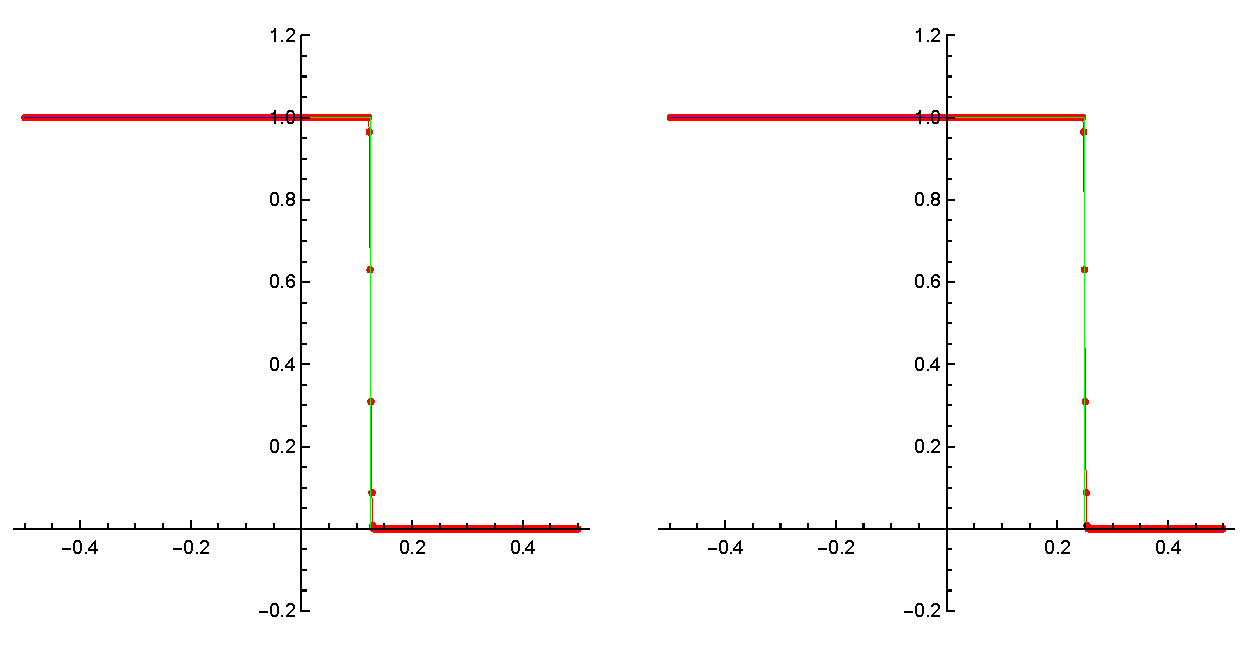
\includegraphics[width=.8\textwidth]{figures/inviscidShock640c4}
	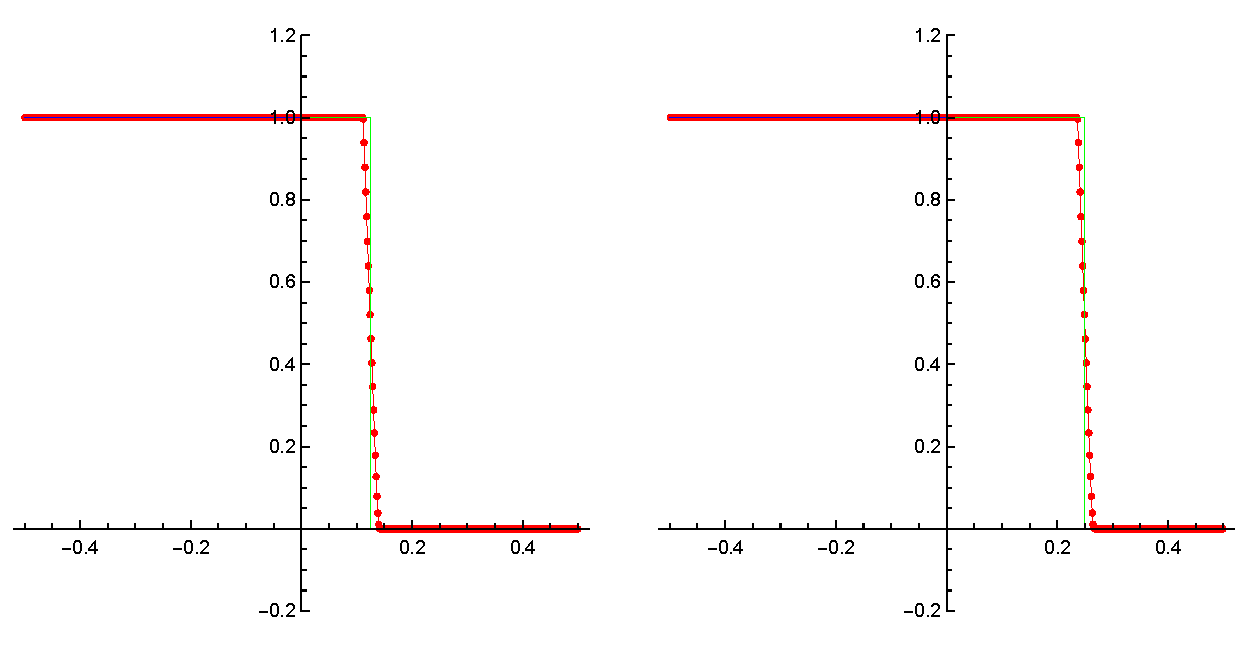
\includegraphics[width=.8\textwidth]{figures/inviscidShock640c32}
	\caption{Results of the $\mathrm{FLIIOE}$(flux limited) scheme \eqref{burgers_limit} with the traveling shock wave solution \eqref{inviscid_shock_sol} of the inviscid Burgers' equation \eqref{inviscid} at time $ t=0.25 $(left) and $ t=0.5 $(right), $ n=640 $ for relatively large time steps $ \tau=4h $(top), $ \tau=32h $(bottom). The initial profile is given in blue, the exact solution in green and the numerical solution in red.}
	\label{fig:fliioe_burg_shock}
\end{figure}

\textbf{Rarefaction wave}. The next example is a solution of \eqref{inviscid} with a discontinuous initial condition
\begin{equation}
	u^0(x) =
	\begin{cases}
		0, &x\leq 0,\nonumber\\
		1, &x>0.\nonumber
	\end{cases}
\end{equation}
A physically relevant weak solution is a rarefaction wave \cite{olv, lev, whitham} for $ t>0 $
\begin{equation}
	\label{inviscid_rare_sol}
	u(t,x) =
	\begin{cases}
		1, &x>t,\nonumber\\
		x/t, &0 \leq x \leq t,\nonumber\\
		0, &x<0.\nonumber
	\end{cases}
\end{equation}
We solved \eqref{inviscid} numerically by \eqref{burgers_limit} on space interval (-0.5, 1.5) and time interval (0, 1). The results are documented in Table ~\ref{tab:fliioe_rare}. The numerical solution is compared visually with the exact one in Figure  ~\ref{fig:fliioe_shock_rare}.
\begin{table}[ht]
	\caption{Report on the $L_1(I,L_1)$ errors of the flux limited $\mathrm{FLIIOE}$ scheme \eqref{burgers_limit} for a rarefaction wave solution \eqref{inviscid_rare_sol} of the inviscid Burgers' equation \eqref{inviscid}. We used time steps $ \tau=h $(top), $ \tau=2h $(bottom).}
	\begin{center} \footnotesize
		\begin{tabular}{|c|c|c|c|c|c|}
			\hline
			$ n $ & $ h $ & $ \tau $ & NTS& $\mathrm{L_1(I,L_1)}$ & EOC \\
			\hline
			\lower.3ex\hbox{80} & \lower.3ex\hbox{0.025} & \lower.3ex\hbox{0.025} & \lower.3ex\hbox{40} & \lower.3ex\hbox{1.63 $10^{-2}$} & \\
			\hline
			\lower.3ex\hbox{160} & \lower.3ex\hbox{0.0125} & \lower.3ex\hbox{0.0125} & \lower.3ex\hbox{80} & \lower.3ex\hbox{8.90 $10^{-3}$} &\lower.3ex\hbox{0.87} \\
			\hline
			\lower.3ex\hbox{320} & \lower.3ex\hbox{0.00625} & \lower.3ex\hbox{0.00625} & \lower.3ex\hbox{160} & \lower.3ex\hbox{4.70 $10^{-3}$}  &\lower.3ex\hbox{0.92}\\
			\hline
			\lower.3ex\hbox{640} & \lower.3ex\hbox{0.003125} & \lower.3ex\hbox{0.003125} & \lower.3ex\hbox{320} & \lower.3ex\hbox{2.42 $10^{-3}$}  &\lower.3ex\hbox{0.96}\\
			\hline \hline
			\lower.3ex\hbox{80} & \lower.3ex\hbox{0.025} & \lower.3ex\hbox{0.05} & \lower.3ex\hbox{20} & \lower.3ex\hbox{2.21 $10^{-2}$} & \\
			\hline
			\lower.3ex\hbox{160} & \lower.3ex\hbox{0.0125} & \lower.3ex\hbox{0.025} & \lower.3ex\hbox{40} & \lower.3ex\hbox{1.22 $10^{-2}$} &\lower.3ex\hbox{0.86} \\
			\hline
			\lower.3ex\hbox{320} & \lower.3ex\hbox{0.00625} & \lower.3ex\hbox{0.0125} & \lower.3ex\hbox{80} & \lower.3ex\hbox{6.58 $10^{-3}$}  &\lower.3ex\hbox{0.89}\\
			\hline
			\lower.3ex\hbox{640} & \lower.3ex\hbox{0.00625} & \lower.3ex\hbox{0.003125} & \lower.3ex\hbox{160} & \lower.3ex\hbox{3.45 $10^{-3}$}  &\lower.3ex\hbox{0.93}\\
			\hline
		\end{tabular}
	\end{center}
	\label{tab:fliioe_rare}
\end{table}
\begin{figure}[H]
	\centering
	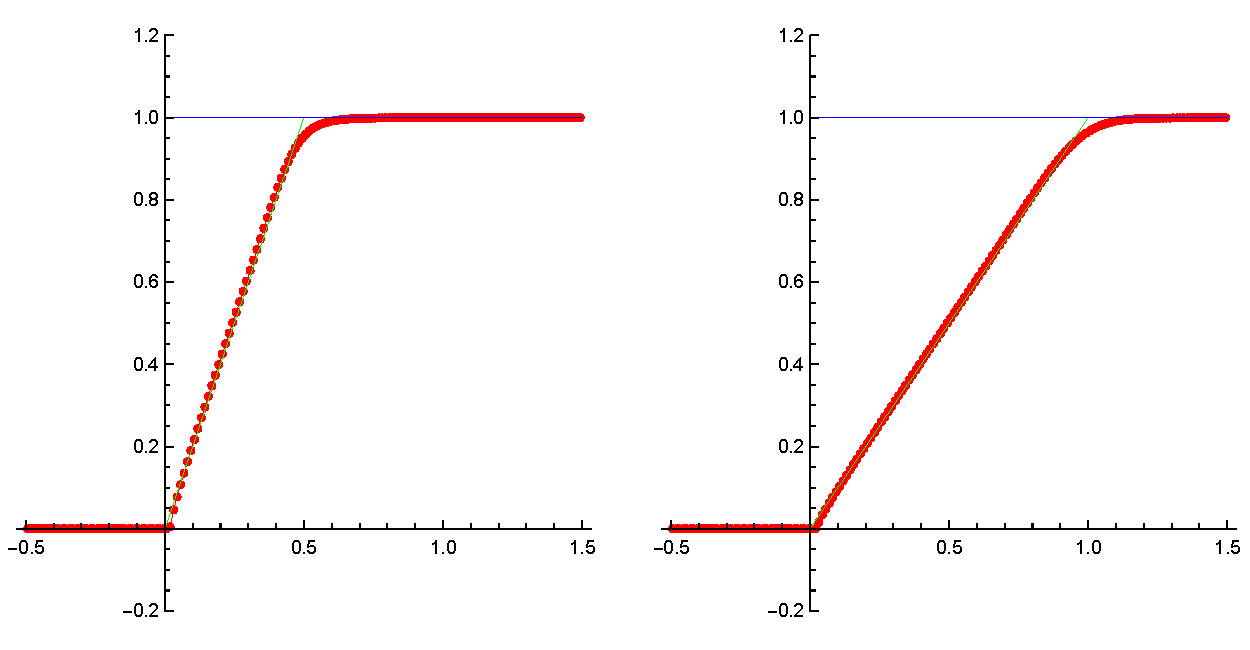
\includegraphics[width=.9\textwidth]{figures/inviscidRare_160_h}
	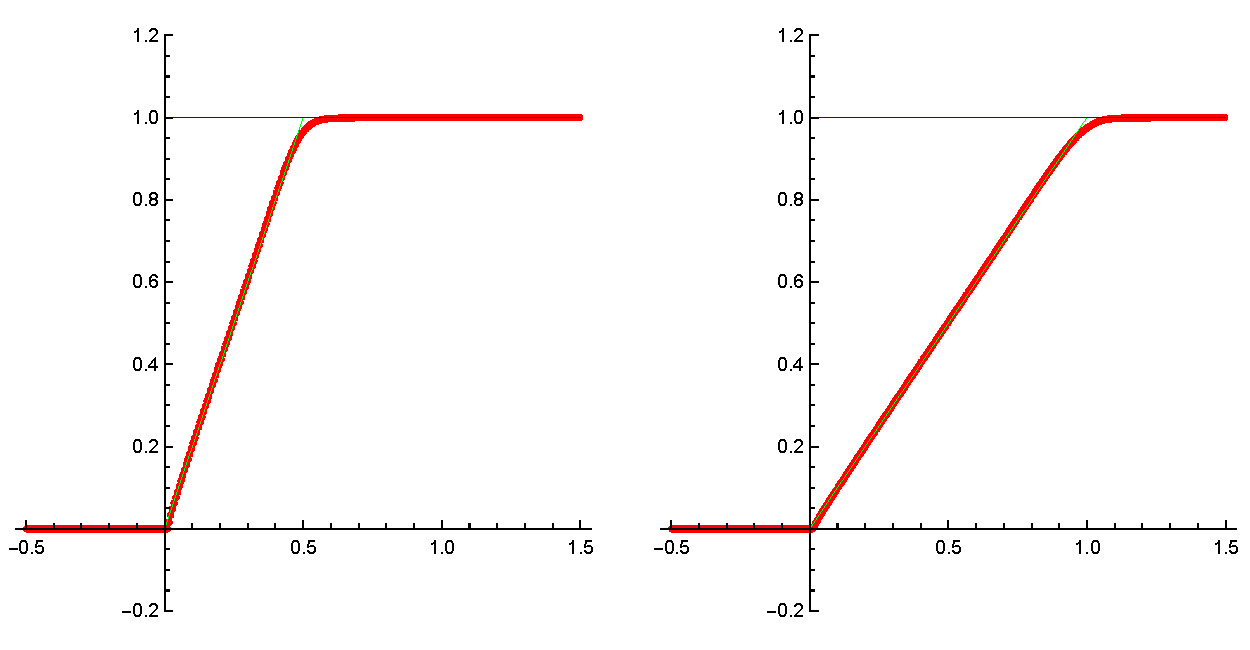
\includegraphics[width=.9\textwidth]{figures/inviscidRare_320_h}
	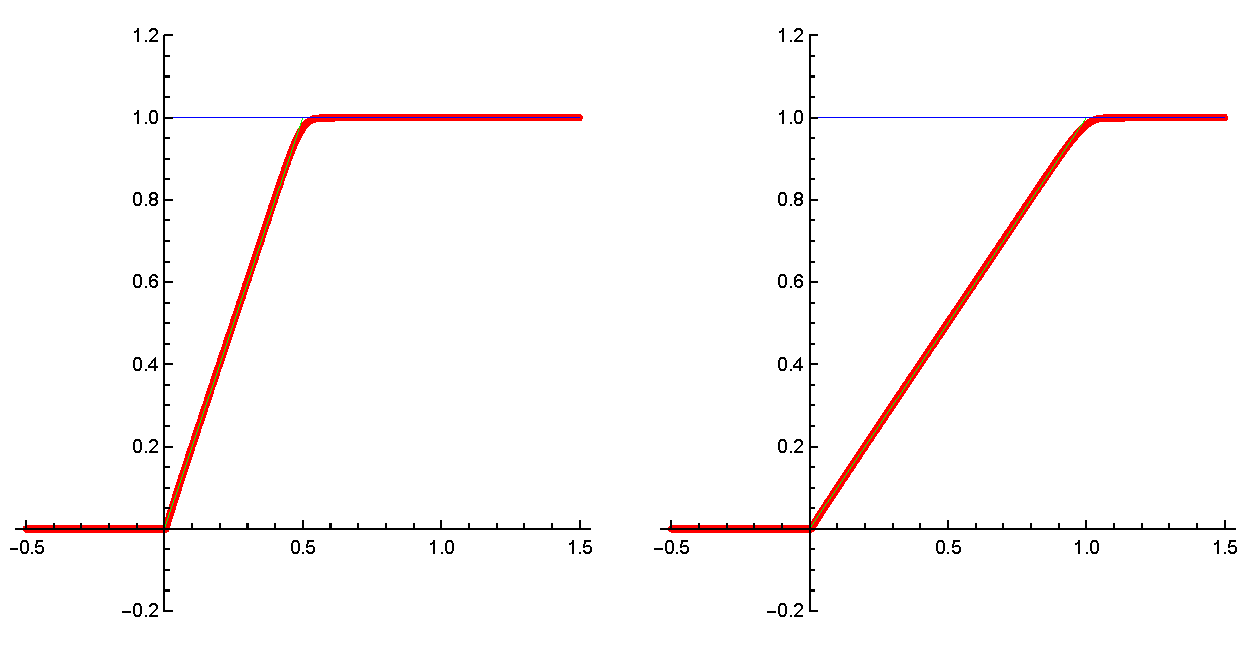
\includegraphics[width=.9\textwidth]{figures/inviscidRare_640_h}
	\caption{Results of the flux limited $\mathrm{FLIIOE}$ scheme \eqref{burgers_limit} for a rarefaction wave solution \eqref{inviscid_rare_sol} of the inviscid Burgers' equation \eqref{inviscid} at time $ t=0.5 $(left) and $ t=1 $(right), $ n=160 $(top), $ n = 320 $(center), $ n = 640 $(bottom) $, \tau=h $. The initial profile is given in blue, the exact solution in green and the numerical solution in red.}
	\label{fig:fliioe_shock_rare}
\end{figure}
\begin{figure}[H]
	\centering
	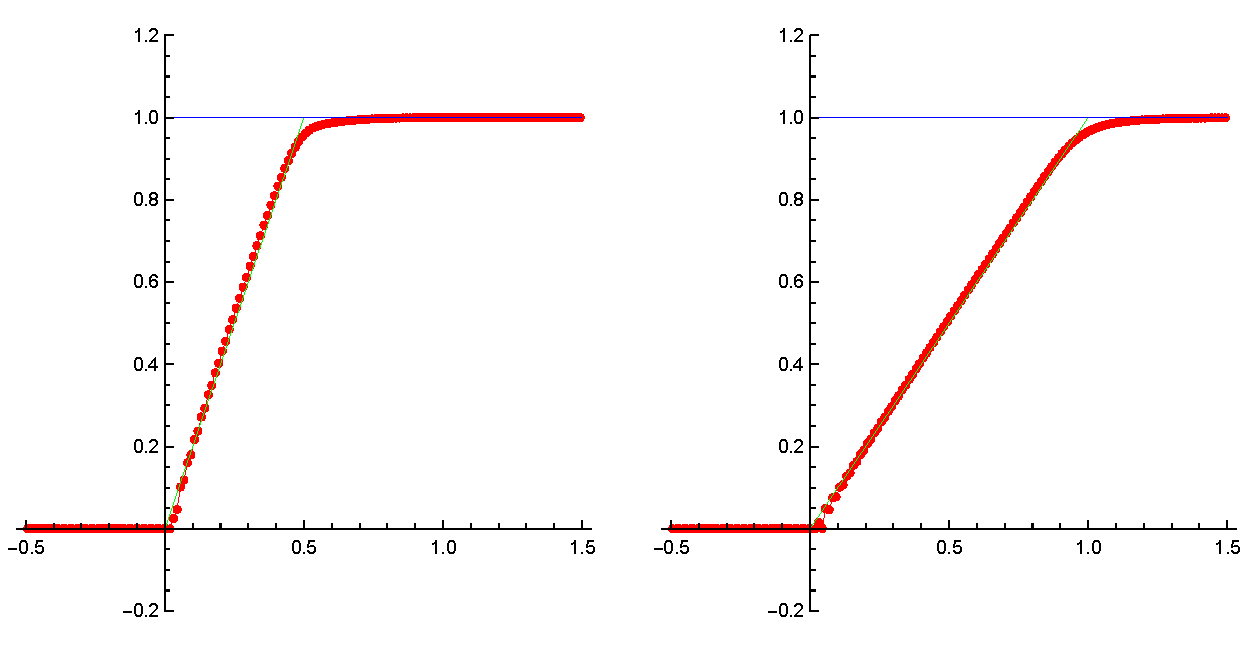
\includegraphics[width=.9\textwidth]{figures/inviscidRare_160_2h}
	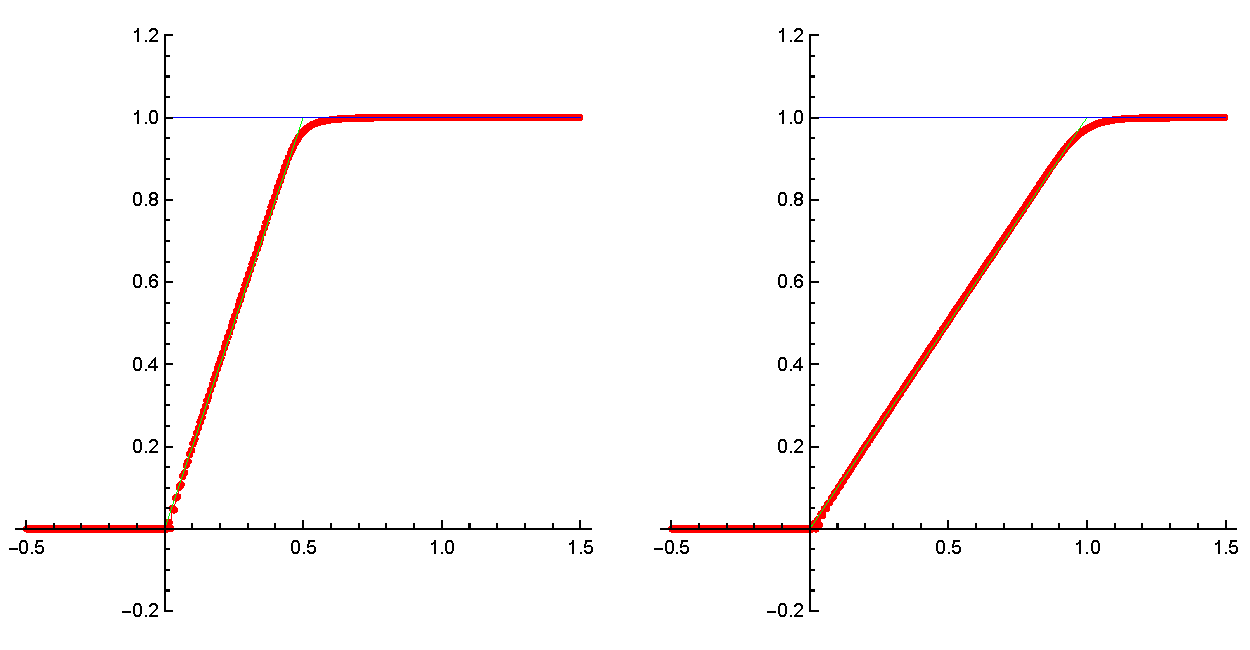
\includegraphics[width=.9\textwidth]{figures/inviscidRare_320_2h}
	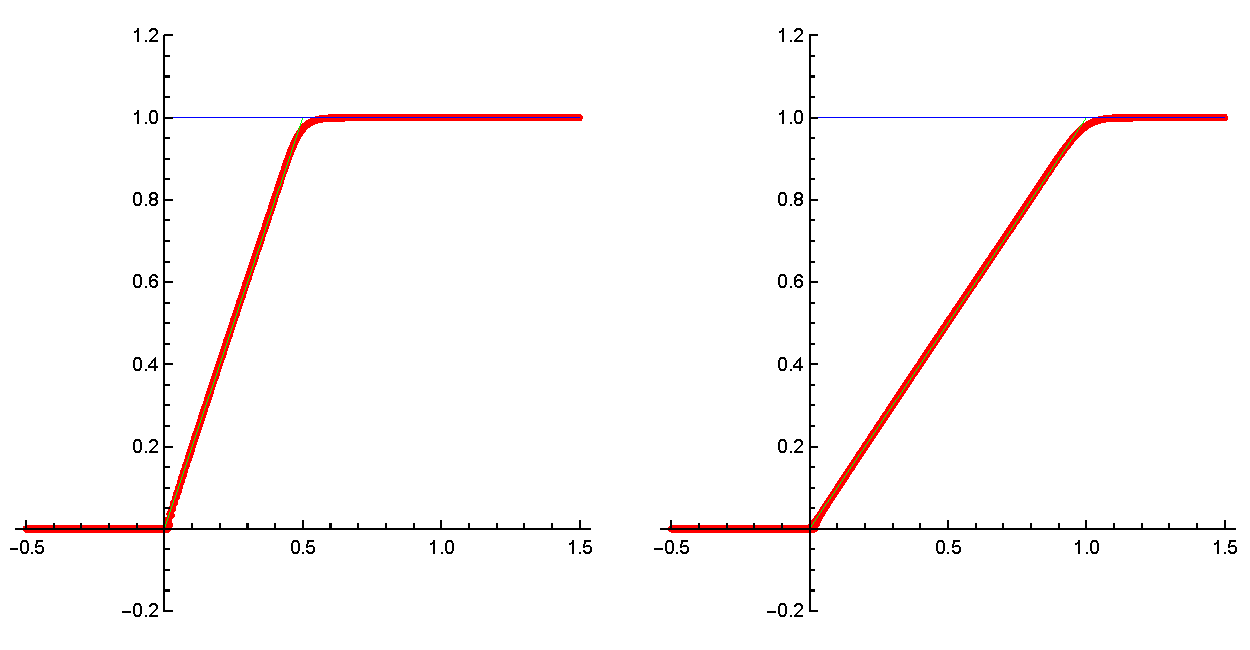
\includegraphics[width=.9\textwidth]{figures/inviscidRare_640_2h}
	\caption{Results of the flux limited $\mathrm{FLIIOE}$ scheme \eqref{burgers_limit} for a rarefaction wave solution \eqref{inviscid_rare_sol} of the inviscid Burgers' equation \eqref{inviscid} at time $ t=0.5 $(left) and $ t=1 $(right), $ n=160 $(top), $ n = 320 $(center), $ n = 640 $(bottom) $, \tau=2h $. The initial profile is given in blue, the exact solution in green and the numerical solution in red.}
	\label{fig:fliioe_shock_rare_2h}
\end{figure}
\newpage
\textbf{Triangular wave}
The third example is another physically relevant weak solution of \eqref{inviscid} \cite{olv, lev, whitham} given for $ t\geq0 $ as
\begin{equation}
	\label{inviscid_triang_sol}
	u(t,x) =
	\begin{cases}
		x/(1+t), &0 \leq x \leq \sqrt{1+t},\nonumber\\
		0, &\mathrm{otherwise}.\nonumber
	\end{cases}
\end{equation}
We solved \eqref{inviscid} numerically by \eqref{burgers_limit} on space interval (-0.5, 1.5) and time interval (0, 1). The results are documented in \ref{tab:fliioe_triang}. The numerical solution is compared visually with the exact one in \ref{fig:fliioe_burg_triang}.
\begin{table}[ht]
	\caption{Report on the $L_1(I, L_1)$ errors of the flux limited $\mathrm{FLIIOE}$ scheme \eqref{burgers_limit} for a triangular wave solution \eqref{inviscid_triang_sol} of the inviscid Burgers' equation \eqref{inviscid}, with time steps $ \tau = h $ in the first 4 rows and $ \tau = 2h $ in the next 4 rows.}
	\begin{center} \footnotesize
		\begin{tabular}{|c|c|c|c|c|c|}
			\hline
			&  & & & $\mathrm{FLIIOE}$ & \\
			\hline
			$ n $ & $ h $ & $ \tau $ & NTS& $\mathrm{L_1(I,L_1)}$ & EOC\\
			\hline
			\lower.3ex\hbox{80} & \lower.3ex\hbox{0.025} & \lower.3ex\hbox{0.025} & \lower.3ex\hbox{40} & \lower.3ex\hbox{1.62 $10^{-2}$} & \\
			\hline
			\lower.3ex\hbox{160} & \lower.3ex\hbox{0.0125} & \lower.3ex\hbox{0.0125} & \lower.3ex\hbox{80} & \lower.3ex\hbox{7.73 $10^{-3}$} &\lower.3ex\hbox{1.07}\\
			\hline
			\lower.3ex\hbox{320} & \lower.3ex\hbox{0.00625} & \lower.3ex\hbox{0.00625} & \lower.3ex\hbox{160} & \lower.3ex\hbox{3.66 $10^{-3}$}  &\lower.3ex\hbox{1.08}\\
			\hline
			\lower.3ex\hbox{640} & \lower.3ex\hbox{0.003125} & \lower.3ex\hbox{0.003125} & \lower.3ex\hbox{320} & \lower.3ex\hbox{1.77 $10^{-3}$}  &\lower.3ex\hbox{1.05}\\
			\hline \hline
			\lower.3ex\hbox{80} & \lower.3ex\hbox{0.025} & \lower.3ex\hbox{0.05} & \lower.3ex\hbox{20} & \lower.3ex\hbox{2.40 $10^{-2}$} &\\
			\hline
			\lower.3ex\hbox{160} & \lower.3ex\hbox{0.0125} & \lower.3ex\hbox{0.025} & \lower.3ex\hbox{40} & \lower.3ex\hbox{1.14 $10^{-2}$} &\lower.3ex\hbox{1.07} \\
			\hline
			\lower.3ex\hbox{320} & \lower.3ex\hbox{0.00625} & \lower.3ex\hbox{0.0125} & \lower.3ex\hbox{80} & \lower.3ex\hbox{5.35 $10^{-3}$}  &\lower.3ex\hbox{1.09}\\
			\hline
			\lower.3ex\hbox{640} & \lower.3ex\hbox{0.00625} & \lower.3ex\hbox{0.003125} & \lower.3ex\hbox{160} & \lower.3ex\hbox{2.66 $10^{-3}$}  &\lower.3ex\hbox{1.01}\\
			\hline
		\end{tabular}
	\end{center}
	\label{tab:fliioe_triang}
\end{table}
\begin{figure}[H]
	\centering
	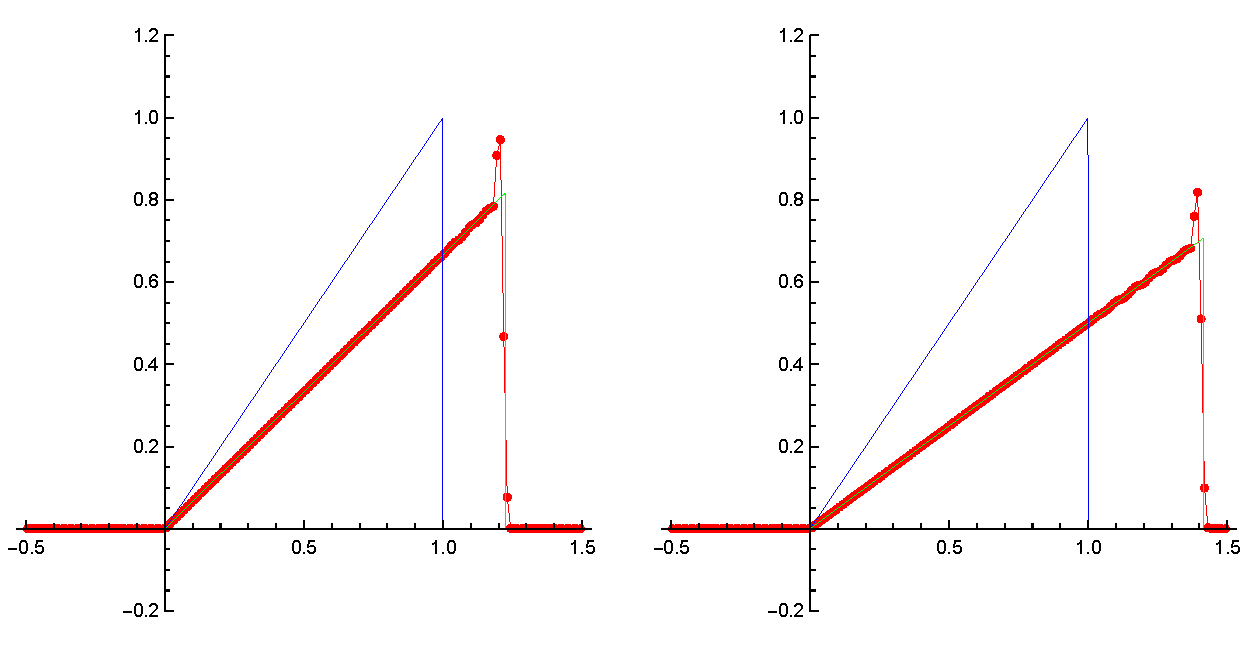
\includegraphics[width=.9\textwidth]{figures/inviscidTriang_160_h}
	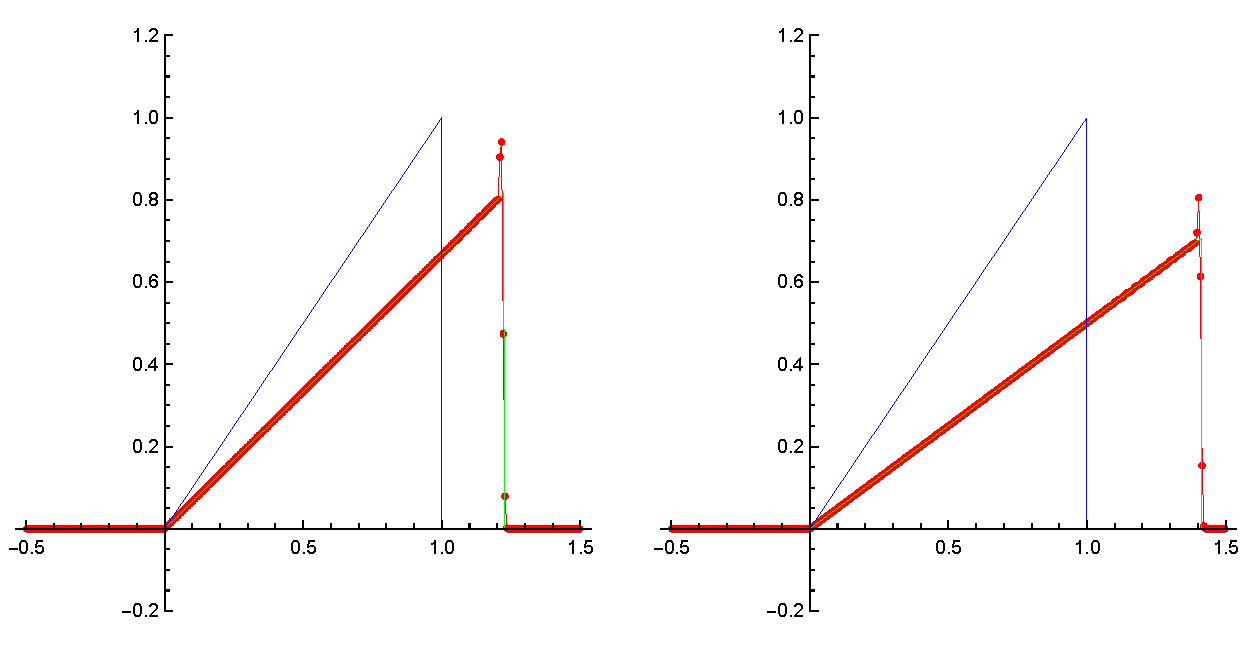
\includegraphics[width=.9\textwidth]{figures/inviscidTriang_320_h}
	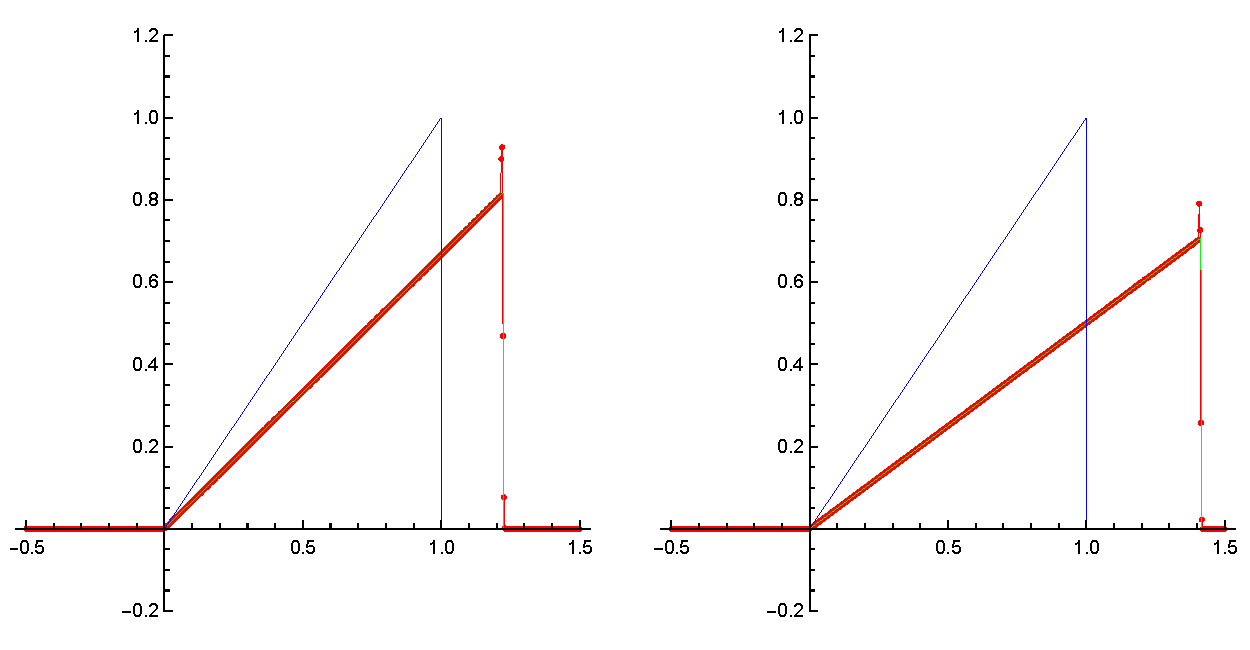
\includegraphics[width=.9\textwidth]{figures/inviscidTriang_640_h}
	\caption{Results of the flux limited $\mathrm{FLIIOE}$ scheme \eqref{burgers_limit} for a triangular wave solution \eqref{inviscid_triang_sol} of the inviscid Burgers' equation \eqref{inviscid} at time $ t=0.5 $(left) and $ t=1 $(right), $ n=160 $(top), $n=320 $(center), $n=640 $(bottom), $ \tau=h $. The initial profile is given in blue, the exact solution in green and the numerical solution in red.}
	\label{fig:fliioe_burg_triang}
\end{figure}
\begin{figure}[H]
	\centering
	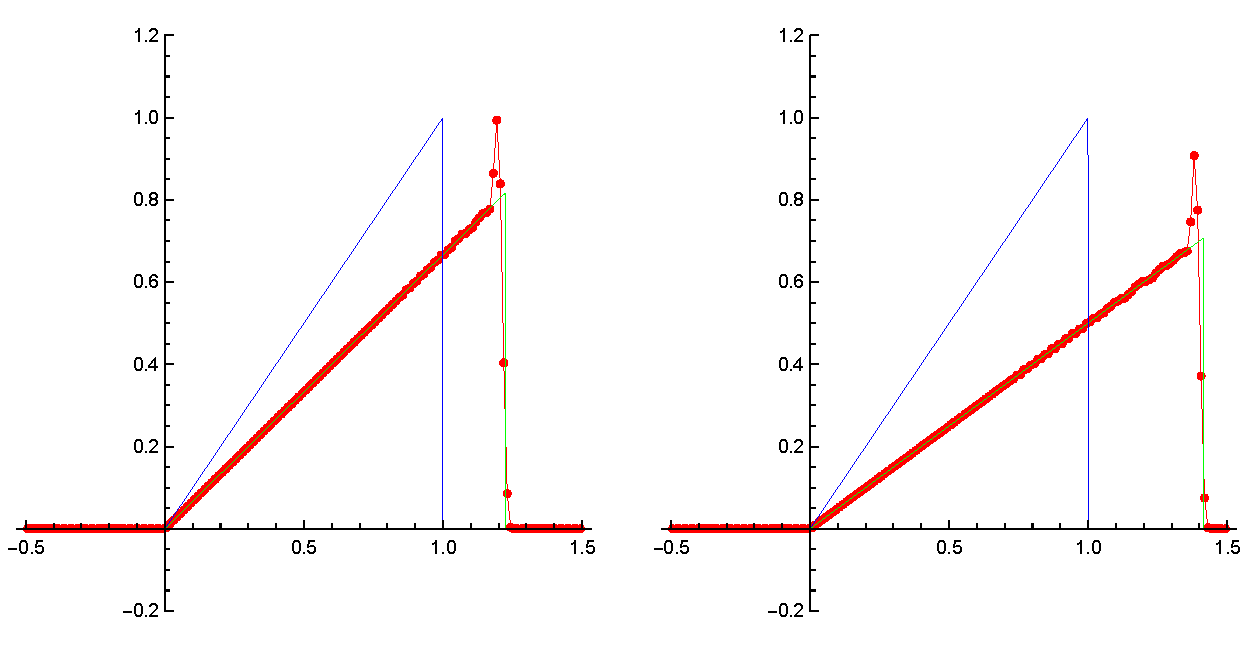
\includegraphics[width=.9\textwidth]{figures/inviscidTriang_160_2h}
	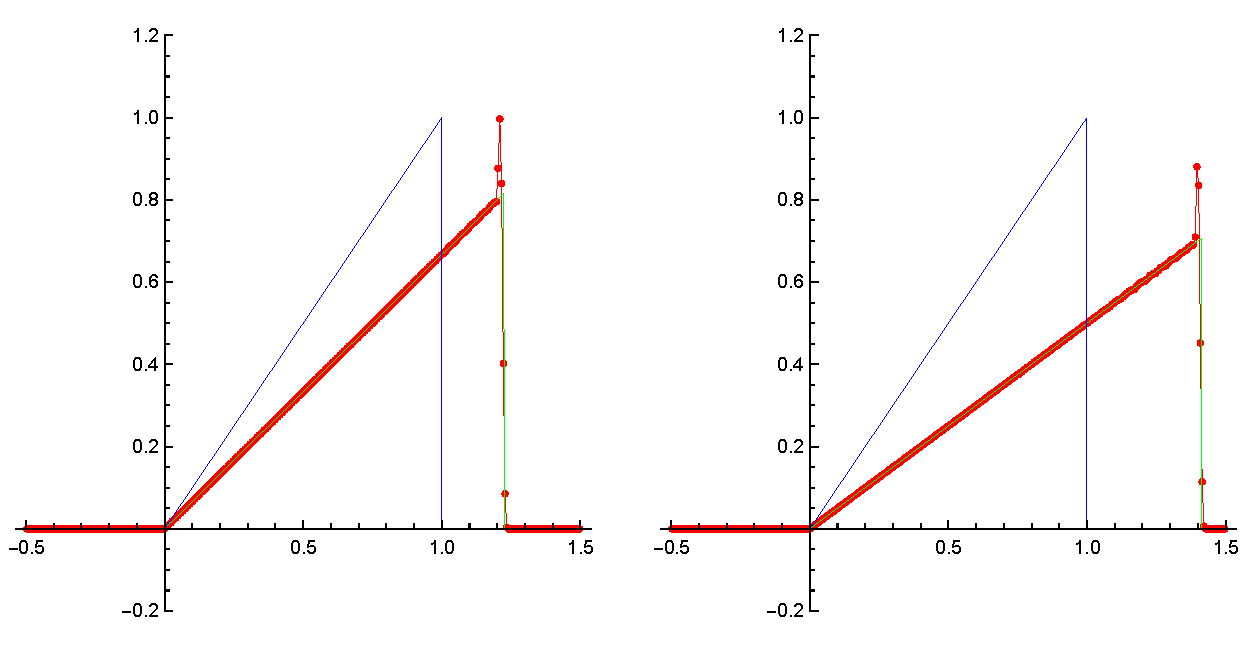
\includegraphics[width=.9\textwidth]{figures/inviscidTriang_320_2h}
	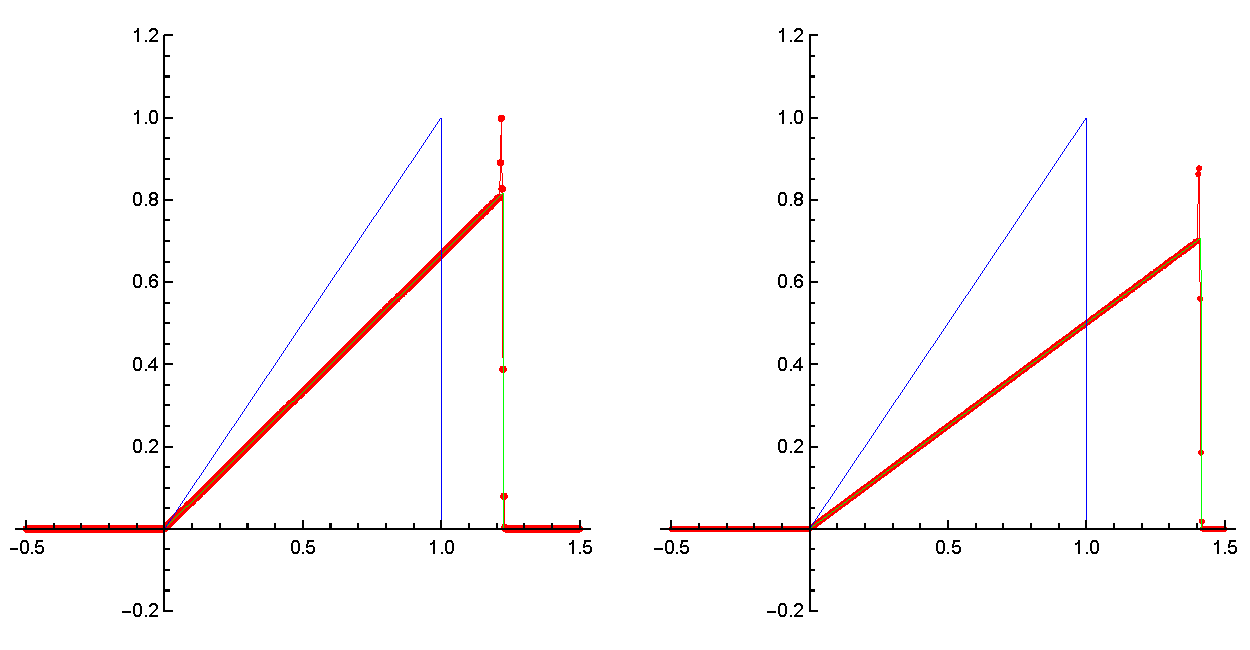
\includegraphics[width=.9\textwidth]{figures/inviscidTriang_640_2h}
	\caption{Results of the flux limited $\mathrm{FLIIOE}$ scheme \eqref{burgers_limit} for a triangular wave solution \eqref{inviscid_triang_sol} of the inviscid Burgers' equation \eqref{inviscid} at time $ t=0.5 $(left) and $ t=1 $(right), $ n=160 $(top), $n=320 $(center), $n=640 $(bottom), $ \tau=2h $. The initial profile is given in blue, the exact solution in green and the numerical solution in red.}
	\label{fig:fliioe_burg_triang_2h}
\end{figure}
\begin{comment}
\begin{figure}[H]
	\centering
	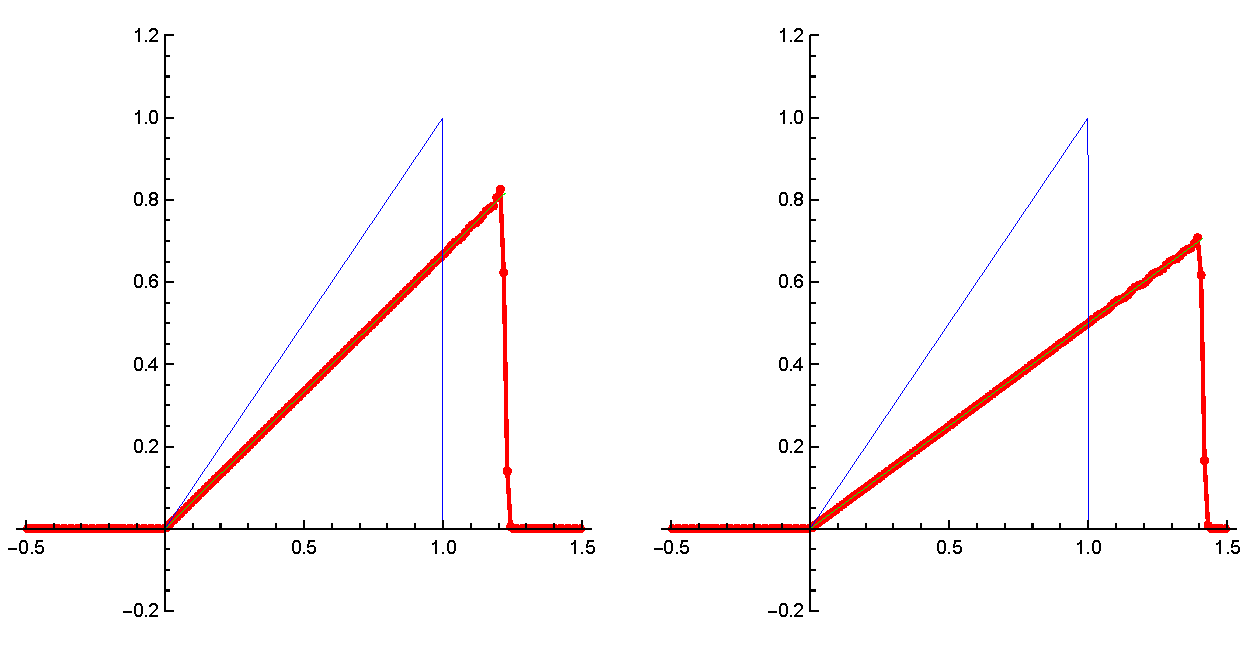
\includegraphics[width=\textwidth]{figures/inviscidTriang_160_h_2nd}
	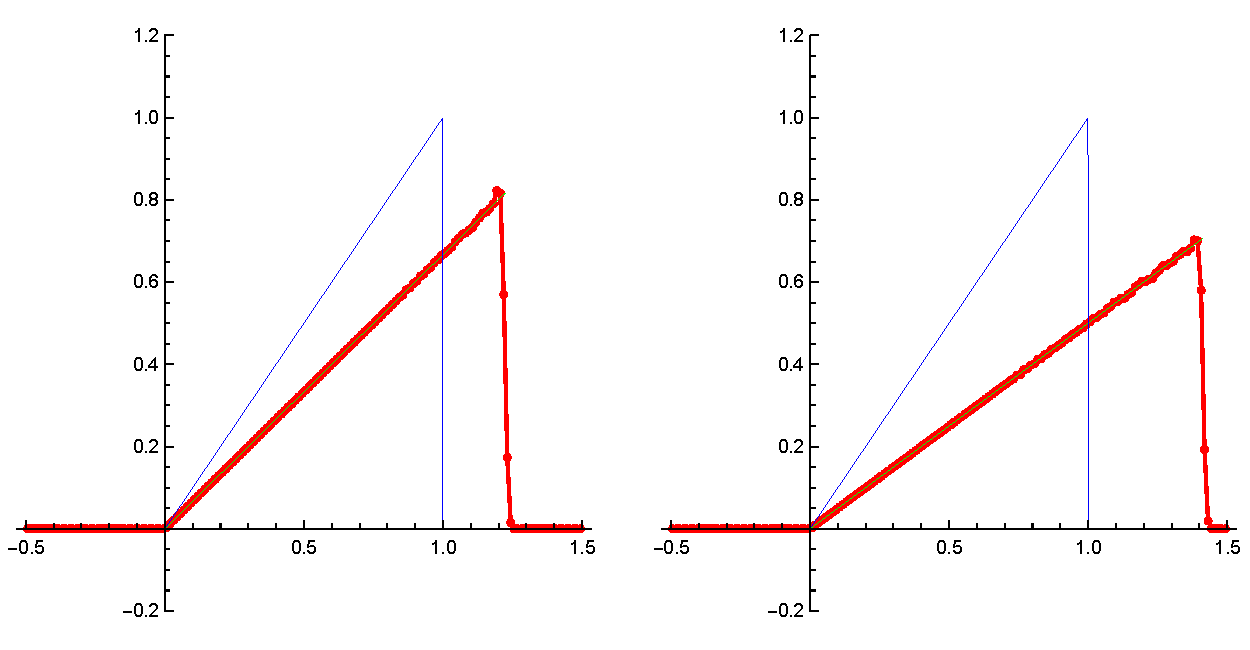
\includegraphics[width=\textwidth]{figures/inviscidTriang_160_2h_2nd}
	\caption{Results of the $\mathrm{FL^2 IIOE}$ flux limited (second approach) scheme for a triangular wave solution of the inviscid Burgers' equation at time $ t=0.5 $(left) and $ t=1 $(right), $ n=160 $. We used time steps $ \tau=h $(top), $ \tau=2h $(bottom). The initial profile is given in black, the exact solution in green and the numerical solution in red.}
	\label{fig:fliioe_burg_triang_2nd}
\end{figure}
\end{comment}
%====================================================================================================================================================
\chapter{Conclusions}
In this work we presented a scheme for solving nonlinear advection-diffusion equations similar to what can be found in \cite{algoritmy}, where for the advection term we applied the IIOE scheme and for the diffusion term we applied the Crank-Nicolson scheme. We tested the performance of the scheme on the viscous Burgers' equation \eqref{burg} and the traffic flow equation \eqref{traffic} by comparing numerical solutions with exact ones. In numerical experiments we can observe second order convergence.

We have shown that the IIOE method can be written in the form of a conservative finite volume method \eqref{finite_volume}, which is crucial for first order scalar conservation laws of the form \eqref{scalar_conservation}. We have shown that on a uniform grid the scheme is formally second order accurate for smooth solutions of scalar conservation laws of the form \eqref{scalar_conservation}. We performed numerical experiments for the inviscid Burgers' equation first in the case of a smooth solution, where the results are in accordance with our theoretical expectations.

For problems, where numerical solutions tend to develop spurious oscillations, a possible flux limiting process were presented, where we want to ensure that the numerical solutions is bounded by some minimum and maximum value. 
%====================================================================================================================================================
\chapter{Thesis objectives and prospective contribution}
\chaptermark{Thesis objectives}
In the future we plan to perform the following tasks:
\begin{itemize}
	%\item Improving the flux-limiting process, extension to 2D, 3D
	\item Generalizing the flux-limiter for arbitrary cases, applications for nonlinear inviscid equations and traffic flow problems
	\item In case of enough time, extension to higher dimensions for other fluid mechanics problems
\end{itemize}
%========================
\end{document}